% ===================================================================
% Arquivo: capitulos/parte-III-pilares/cap-10-perda-binaria.tex
% ===================================================================

\chapter{Funções de perda para classificação}%
\label{cap:perda-classificacao}

\section{Exemplo ilustrativo: cara ou coroa}

Imagine que você decidiu apostar com seus amigos qual lado uma moeda irá cair. Contudo, você decidiu fazer um jogo mais complicado, ao invés de decidir apenas entre cara e coroa, serão analisadas probabilidades. Probabilidades próximas de 0 indicam que irá a nova rodada resultará em cara, já as próximas de 1 são referentes a coroa. Uma probabilidade muito alta, como 0,89 pode ser ser muito bom se cair coroa, pois irá ganhar mais pontos. Contudo, se cair cara, o prejuízo será grande, estará sendo feito um erro confiante.

Nesse jogo, a entropia-binária cruzada é a juíza, é ela quem dita quem irá receber ou perder muitos pontos. Ela tem como principal função ser utilizada em problemas nos quais temos duas classes, como o do jogo da moeda. Ela também tem a tendência de penalizar mais as predições confiantes, gerando gradientes maiores em magnitude e até mesmo causar problemas de gradientes explosivos se não for utilizada da forma correta.

\section{Funções de perda para classificação binária}

\subsection{Entropia-cruzada binária (BCE)}%
\index{Funções de Perda!Entropia-cruzada binária (BCE)}%
\label{sec:binary-cross-entropy}

A história da origem da \textbf{entropia-cruzada binária}, também chamada de \textbf{\textit{binary cross-entropy}} (\textbf{BCE}), tem origem no final dos anos 1940, mais especificadamente com o avanço da teoria da comunicação. Em \textit{A Matematical Theory of Comunication}, \textcite{EntropyShannon} estudava sobre formas eficientes de comunicação, em um dos momentos do artigo ele define o conceito de Entropia, como uma medida de incerteza, ou da ``escolha'', associada a um conjunto de eventos com determinada probabilidades. A Entropia de Shannon, definida pela Equação~\ref{eq:entropia-de-shannon}, torna-se a peça central para descrever a diversas funções, sendo uma delas a divergência KL.

\begin{equacaodestaque}{Entropia de Shannon}
    H(p) = - k \sum_{i = 1}^{n} p_i \log pi%
    \label{eq:entropia-de-shannon}
\end{equacaodestaque}

Passado alguns anos, outros autores já estavam trabalhando com o conceito de entropia de Shannon. \textcite{KullbackLeiblerDivergence} em \textit{On Information and Sufficiency} expandem o conceito de entropia para lidar com casos contínuos além de introduzirem uma medida para comparar duas distribuições de probabilidades $p$ e $q$, chamando-a de informação para discriminação. Essa medida, representada na Equação~\ref{eq:kl-divergence},  futuramente passou a ser conhecida com divergência de Kullback-Leibler (\textit{KL Divergence}).

\begin{equacaodestaque}{Divergência de Kullback-Leibler}
    I(1:2) = I_{1:2}(X) = \int f_1 (x) \log \frac{f_1(x)}{f_2 (x)} d \lambda (x)%
    \label{eq:kl-divergence}
\end{equacaodestaque}

A divergência KL mede a ``perda'' ou o ``excesso'' de informação quando é utilizada uma distribuição $q$ para aproximar a distribuição real $q$. Da definição da divergência KL podemos chegar na entropia-cruzada, tendo ela, poderemos escrever a BCE.

Na Equação~\ref{eq:kl-divergence}, utilizamos as propriedades do logaritmo para reescrever da divergência KL em

\[
    I(1:2) = I_{1:2}(X) = \int f_1 (x) (\log f_1 (x) - \log f_2 (x)) d\lambda (x)
\]

Em seguida, utilizando a propriedade distributiva, nós expandimos a equação, encontrando

\[
    I(1:2) = I_{1:2}(X) = \int f_1 (x) \log f_1 (x) - f_1 (x) \log f_2 (x) d \lambda (x)
\]

Dessa nova equação, separamos a integral em duas diferentes, chegando em

\[
    I(1:2) = \int f_1 (x) \log f_1 (x) d\lambda (x) - \int f_1 (x) \log f_2 (x) d\lambda(x)
\]

O primeiro termo é quase igual a fórmula proposta por Shannon para a entropia, exceto por um sinal de menos. Assim, o primeiro termo pode ser reescrito como $-H(f_1)$. Já o segundo termo é a própria definição de entropia-cruzada entre $f_1$ e $f_2$, portanto $H(f_1, f_2)$. A definição de entropia-cruzada está descrita na Equação~\ref{eq:cross-entropy}.

\begin{equacaodestaque}{Entropia-cruzada}
    H(f_1, f_2) = \int f_1 (x) \log f_2 (x) d\lambda(x)%
    \label{eq:cross-entropy}
\end{equacaodestaque}

Com base nesses dois termos, o da entropia-cruzada, e o da entropia de Shannon, reescrevemos mais uma vez a definição da Equação~\ref{eq:kl-divergence}, agora utilizando os termos resumidos. Temos então

\[
    I(1:2) = H(f_1, f_2) - H(f_2)
\]

que também pode ser escrita como

\[
    D_{KL} (f_1 || f_2) = H(f_1, f_2) - H(f_1)
\]

Dizemos que a divergência de Kullback-Leibler é a diferença entre a entropia-cruzada e a entropia de Shannon. Reescrevendo a equação mais uma vez é encontramos

\[
    H(f_1, f_2) = H(f_1) + I(1:2)
\]

Essa equação nos diz que o custo real de codificar os dados usando um modelo imperfeito $H(f_1, f_2)$ é igual ao custo de codificar usando um modelo perfeito $H(f_1)$ mais uma penalidade extra pela diferença entre o modelo perfeito e imperfeito. Concluímos que minimizar a divergência KL, é o mesmo que minimizar a entropia-cruzada em cenários de aprendizado de máquina. Como a Entropia dos dados reais é uma constante, ao reduzir a entropia-cruzada, é ao mesmo tempo forçar a redução da divergência KL, aproximando mais o modelo dos dados da realidade.

A partir desses dois conceitos chegamos finalmente na entropia-cruzada binária, o tópico principal desta seção. A BCE é dada pela Equação \ref{eq:binary-cross-entropy}. A sua fórmula calcula a perda de forma elegante, aplicando o cálculo de duas entropias cruzadas. A primeira, $y \log(\hat{y})$, calcula a distância de uma classe 0 com o retorno do modelo $\hat{y}$. A segunda, $(1 - y) \log(1 - \hat{y})$, calcula a distância para os casos em que está sendo analisada a classe 1. Dessa forma, em um cenário em que o resultado é a classe 0, a primeira entropia-cruzada é toda multiplicado por zero, sendo eliminada da fórmula. O mesmo vale para quando o resultado é a classe 1, em que a segunda entropia-cruzada passa a ser zero.

\begin{equacaodestaque}{Entropia-cruzada binária}
    \mathcal{L}_{\text{bce}} (y, \hat{y}) = -[y \log(\hat{y}) + (1 - y) \log(1 - \hat{y})]%
    \label{eq:binary-cross-entropy}
\end{equacaodestaque}

Em que

\begin{description}[style=sameline, leftmargin=1.5em, font=\bfseries\color{black}] 
    \item[$y$] representa os rótulos dos dados, segue o formato $y \in {0, +1}$;
    \item[$\hat{y}$] representa a probabilidade prevista para a amostra.
\end{description}

Assim como visto no Capítulo~\ref{cap:perda-regressao}, neste capítulo representaremos as perdas para uma única predição. Contudo, no cenário de aprendizado de máquina, também podemos representar as perdas como a média do cálculo individual das perdas, como em

\[
    \mathcal{L}_{\text{bce}} = \frac{1}{N} \sum_{i=1}^{N} [y_i \log(\hat{y}_i) + (1 - y_i) \log(1 - \hat{y}_i)]
\]

A BCE é utilizada em de aprendizado de máquina há um bom tempo. Um dos trabalhos que cita o uso dessa função para ser utilizada classificação binária é o \textit{Connectionist Learning Procedures}, nele, \textcite{HintonConnectionist} explica que ao minimizar a entropia-cruzada binária para as distribuições do resultado desejado e o atual resultado era semelhante a maximizar a a verossimilhança do modelo gerar as saídas corretas.

O gráfico da entropia-cruzada binária apresenta duas curvas distintas, como evidenciado pela Figura~\ref{fig:binary-cross-entropy}. A primeira curva é responsável por indicar a probabilidade prevista pelo modelo para a classe zero. Enquanto a segunda, é referente à probabilidade prevista para a classe um. Elas são dependentes uma da outra, dado que a probabilidade para uma determinada classe será sempre 1 menos a probabilidade prevista para a outra classe.

\begin{figure}
    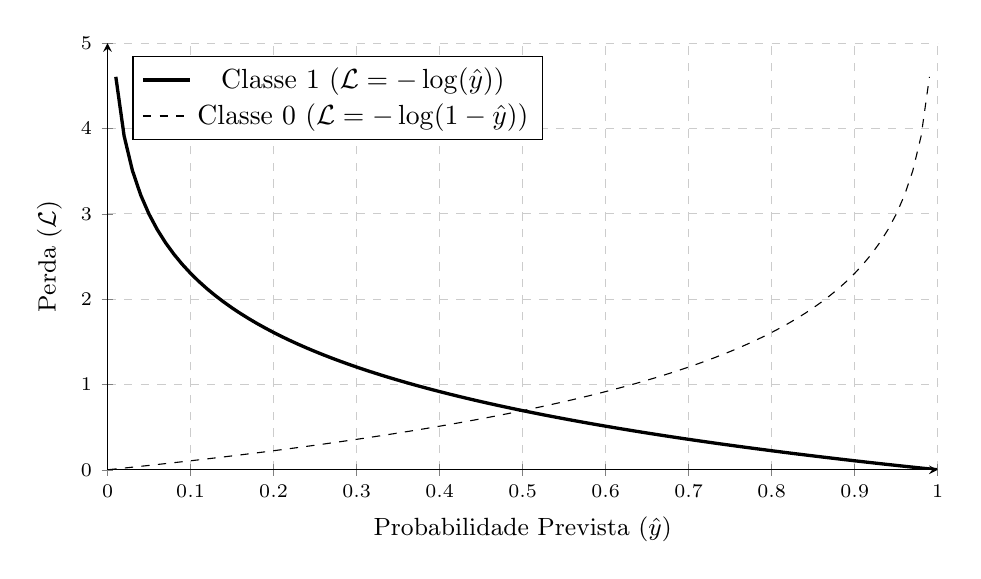
\begin{tikzpicture}
        \begin{axis}[
            xlabel={Probabilidade Prevista ($\hat{y}$)},
            ylabel={Perda ($\mathcal{L}$)},
            axis lines=left,            
            grid=major,                
            grid style={dashed, gray!40},  
            xmin=0, xmax=1,             
            ymin=0, ymax=5,             
            legend pos=north west,     
            width=\linewidth,
            height=7cm,
            title style={font=\bfseries},
            label style={font=\small},
            tick label style={font=\scriptsize}
        ]
            \addplot[
                domain=0.01:0.999,
                samples=100,
                color=black,
                very thick
            ] {-ln(x)};
            \addlegendentry{Classe 1 ($\mathcal{L} = -\log(\hat{y})$)}

            \addplot[
                domain=0.001:0.99,
                samples=100,
                color=black,
                dashed
            ] {-ln(1-x)};
            \addlegendentry{Classe 0 ($\mathcal{L} = -\log(1-\hat{y})$)}
            
        \end{axis}
    \end{tikzpicture}
    \caption{Visualizações da função de perda entropia-cruzada binária no plano.}
    \label{fig:binary-cross-entropy}
    \fonte{O autor (2025).}
\end{figure}

\subsubsection*{Características da entropia-cruzada binária}

\begin{description}[style=sameline, leftmargin=1.5em, font=\bfseries\color{black}] 
    \item[Continuidade, suavidade e diferenciabilidade:] A BCE é uma função de classe $C^{\infty}$, \textbf{infinitamente diferenciável} no domínio aberto $\hat{y} \in (0, 1)$ (ver Apêndice~\ref{ap:deducoes-perdas-derivadas-da-kl-divergence}). Podemos garantir que a saída do modelo esteja em um intervalo $(0,1)$ utilizando a função de ativação sigmoide logística na última camada. Fazendo isso, asseguramos a diferenciabilidade da perda, facilitando a otimização por gradiente.
    \item[Convexidade:] A BCE é \textbf{convexa} em relação predições $\hat{y}$ (ver Apêndice~\ref{ap:deducoes-perdas-derivadas-da-kl-divergence}). Sendo uma função convexa, a perda apresentará apenas um ponto de mínimo global, com formato favorável a utilização de otimizadores baseados em gradiente. Contudo, não é possível garantir que a BCE continuará sendo convexa em modelos de aprendizado profundo, devido às transformações não-lineares que ocorrem nas camadas.
    \item[Robustez:] A BCE não é Lipschitz-contínua, sendo \textbf{sensível a erros confiantes} (ver Apêndice~\ref{ap:deducoes-perdas-derivadas-da-kl-divergence}). Diferente das perdas para regressão, que podem ser sensível a \textit{outliers}, as perdas de classificação podem ser sensíveis a erros confiantes. Dado que a BCE possui a tendência de punir agressivamente erros confiantes, isso gera gradientes grandes em magnitude, podendo ocasionar explosões de gradientes.
    \item[Origem na teoria da informação:] Como foi visto no início da seção a BCE está estritamente ligada com o conceito de Entropia de Shannon. \textcite{LossesArticle} explicam que essa função mede a distância entre duas distribuições de Bernoulli, a distribuição real $P(y)$ e a distribuição de predições $Q(y)$.
    \item[Pune erros confiantes:] Quando $\hat{y}$ é perto de 1, mas o valor real é o oposto, neste caso, $y = 0$, o termo logarítmico $\log(\hat{y})$ ou $\log(1 - \hat{y})$ fica grande em magnitude, penalizando muito os erros confiantes. Essa relação também vale para o contrário, em que $\hat{y}$ é perto de 0, mas $y = 1$.
    \item[Desbalanceamento de classes:] Em cenários que uma classe é significativamente mais presente que outra, a BCE pode gerar modelos enviesados \parencite{LossesArticle}. Como solução, é possível utilizar a função de perda entropia-cruzada binária ponderada (ver Seção~\ref{sec:binary-weighted-cross-entropy}), essa função busca resolver o problema do desbalanceamento de classes aplicando pesos para as diferentes classes do problema estudado.
\end{description}

\subsubsection*{Gradiente da entropia-cruzada binária}

A derivada parcial da entropia-cruzada em relação à predição está na Equação~\ref{eq:binary-cross-entropy-derivada}. É a partir dela que é formado o vetor gradiente, que será retropropagado por toda a rede, da camada de saída até a camada de entrada, ajustando os parâmetros do modelo.

\begin{equacaodestaque}{Gradiente da entropia-cruzada binária em relação à predição}
    \nabla_{\hat{y}} \mathcal{L}_{\text{bce}} (y, \hat{y}) = \frac{\hat{y} - y}{\hat{y}(1 - \hat{y})}
    \label{eq:binary-cross-entropy-derivada}
\end{equacaodestaque}

Essa equação explicita o motivo da BCE não ser Lipschitz-contínua, pois quando $\hat{y}$ for um valor muito pequeno e $y = 1$ temos

\[
    \lim_{\hat{y} \to 0} \frac{\hat{y} - 1}{\hat{y}(1 - \hat{y})} = - \infty
\]

Analogamente, quando $\hat{y}$ for um valor próximo de 1 e $y = 0$ temos

\[
    \lim_{\hat{y} \to 0} \frac{1}{(1 - \hat{y})} = + \infty
\]

Essa situação na qual ocorre a explosão do gradiente está apresentada na Figura~\ref{fig:binary-cross-entropy}. Existem duas assíntotas verticais em 0 e 1 no gráfico, indicando que o gradiente cresce indefinidamente quando se aproxima desses pontos.

\begin{figure}[h!]
    \centering
    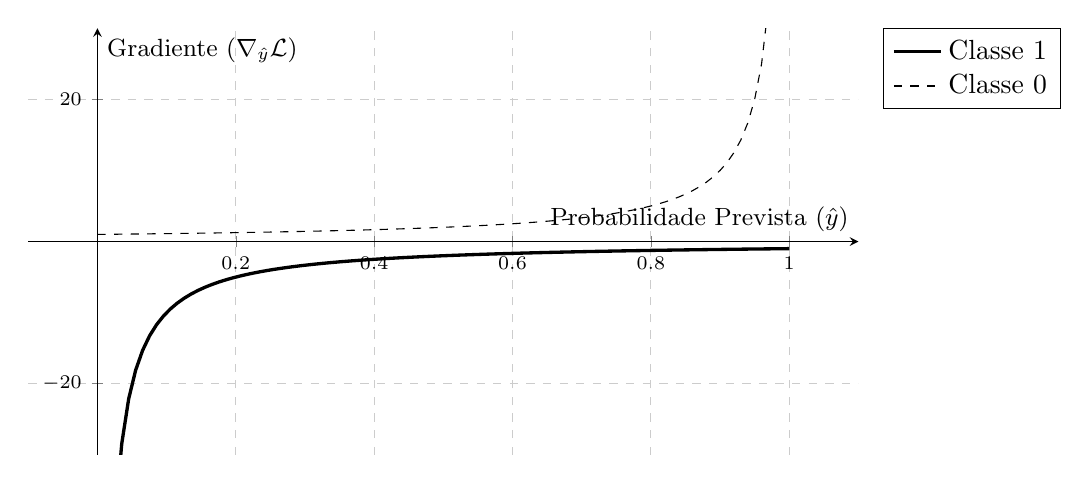
\begin{tikzpicture}
        \begin{axis}[
            xlabel={Probabilidade Prevista ($\hat{y}$)},
            ylabel={Gradiente ($\nabla_{\hat{y}} \mathcal{L}$)},
            axis lines=middle,
            grid=major,
            grid style={dashed, gray!40},
            xmin=-0.1, xmax=1.1,
            ymin=-30, ymax=30, % Aumentar o range do y para ver a assíntota
            legend pos=outer north east,
            width=\linewidth,
            height=7cm,
            title style={font=\bfseries},
            label style={font=\small},
            tick label style={font=\scriptsize}
        ]
            % Derivada para a classe real y=1
            % Fórmula: (y_hat - 1) / (y_hat * (1 - y_hat)) = -1 / y_hat
            \addplot[
                domain=0.005:1, % Domínio para evitar divisão por zero
                samples=100,
                color=black,
                very thick
            ] {-1/x};
            \addlegendentry{Classe 1}

            % Derivada para a classe real y=0
            % Fórmula: (y_hat - 0) / (y_hat * (1 - y_hat)) = 1 / (1 - y_hat)
            \addplot[
                domain=0:0.99, % Domínio para evitar divisão por zero
                samples=100,
                color=black,
                dashed
            ] {1/(1-x)};
            \addlegendentry{Classe 0}
            
        \end{axis}
    \end{tikzpicture}
    \caption{Visualização do gradiente de perda entropia-cruzada binária.}
    \label{fig:binary-cross-entropy-derivada}
    \fonte{O autor (2025).}
\end{figure}

Uma maneira de tratar a explosão do gradiente ao calcular a derivada da perda é utilizar a sigmoide na camada de saída. Visto que a sigmoide irá garantir que as saídas do modelo estejam no intervalo $[0, 1]$, além disso, ao combinar essa função de ativação com a BCE é garantido um cálculo mais simples para o gradiente. Essa nova derivada está representada na Equação~\ref{eq:bce-derivada-com-sigmoide}, o gradiente torna-se a diferença da predição com o valor real. Esse gradiente será sempre limitado, pois $\hat{y}$ está entre 0 e 1 e $y$ é 1 ou 0, de forma que o gradiente estará no intervalo $[-1, 1]$.

\begin{equacaodestaque}{Gradiente da entropia-cruzada binária em relação à predição com sigmoide logística}
    \nabla_{\hat{y}} \mathcal{L}_{\text{bce}} (y, \hat{y}) = \hat{y} - y
    \label{eq:bce-derivada-com-sigmoide}
\end{equacaodestaque}

Quando derivamos a perda em relação a \textit{logit} encontramos a mesma equação da derivada do erro quadrático médio, utilizado para regressão linear. Isso mostra que a regressão linear, que utilizada o MSE, e a regressão logística, que utiliza a BCE, estão relacionadas. A única diferença é a função de ligação em cada uma delas, para o MSE é utilizada a função identidade, e para a BCE é utilizada a sigmoide logística.

Na prática, o que bibliotecas como PyTorch fazem é aplicar a sigmoide logística junto com a BCE em apenas uma operação. A função BCEWithLogitsLoss do \textcite{PyTorchBCEWithLogitsLoss} utiliza um truque matemático conhecido como Log-Sum-Exp, no qual o logaritmo natural e a sigmoide são fundidos em apenas uma expressão. Isso resulta em uma equação estável, que contribui para reduzir os problemas de explosão de gradientes no cálculo da derivada da perda. Essa expressão utilizada pelo PyTorch está na Equação 

\begin{equacaodestaque}{BCEWithLogitsLoss}
    \mathcal{L}_n = -[y_n \log(\sigma(x_n)) + (1 - y_n) \log(1 - \sigma(x_n))]
    \label{eq:BCEWithLogitsLoss}
\end{equacaodestaque}


\subsubsection*{Aplicações da entropia-cruzada binária}%
\index{Aplicações práticas! Entropia Cruzada Binária}

\begin{description}[style=sameline, leftmargin=1.5em, font=\bfseries\color{black}] 
    \item[Detecção de ataques em reconhecimento facial (Segurança):] \textcite{cai2024sadaptergeneralizingvisiontransformer} adaptam um \textit{vision transformer} (ViT) para lidar com ataques de apresentação (\textit{face Anti-Spoofing} (FAS)), como existem duas classes para serem identificadas, real ou falso, a BCE é utilizada como função de perda.
    \item[Classificação de textos ofensivos com análise de sentimento (Área):] \textcite{islam2024leveragingsentimentoffensivetext} utiliza análise de sentimentos para classificar textos do \textit{dataset} OLID entre ofensivos e não ofensivos, o autor faz uso da BCE para função de perda.
    \item[Predição da função de proteínas (Bioinformática):] \textcite{chervov2024protboostproteinfunctionprediction} combina \textit{gradient boosting} com redes neurais em grafo (GNNs) para prever a função de proteínas, o autor utiliza a BCE em conjunto com a \textit{soft F1 loss} como funções de perda.
\end{description}

\medskip

Como dito na seção de propriedades da perda BCE, ela apresenta a tendência de enviesar o aprendizado do modelo em cenários em que um classe é mais comum que a outra. Nestes casos, uma solução é utilizar a sua versão ponderada, a entropia-cruzada binária ponderada.

\subsection{Entropia-cruzada binária ponderada (WBCE)}%
\index{Funções de Perda!Entropia-cruzada binária ponderada (WBCE)}%
\label{sec:binary-weighted-cross-entropy}

Considere o seguinte cenário: está sendo criado um modelo para detecção de câncer de pele em um dataset no qual 90\% das imagens são de pessoas saudáveis. O modelo criado está excelente em predizer se uma pessoa está saudável, de forma que acerta todas as predições para a classe saudável e erra todas as predições para câncer de pele. Na prática, ele está com uma acurácia de 90\%, o que é muito bom, exceto pelo fato de que ele não aprendeu a detectar nenhum câncer. 

Utilizar a BCE com \textit{datasets} com classes desbalanceadas pode causar modelos enviesados, ótimos para reconhecer uma das classes mas péssimos para reconhecer a outra classe. Uma solução é adicionar pesos para as classes, a classe em maior presença recebe um peso baixo e a classe em desvantagem numérica recebe um peso alto. Essa é a solução por trás da \textbf{entropia-cruzada binária ponderada}, também chamada de \textbf{\textit{weighted binary cross-entropy}} (\textbf{WBCE}).

A WBCE adiciona pesos a cada uma das classes, como na Equação~\ref{eq:binary-weighted-cross-entropy}. A classe menos presente recebe um peso maior, consequentemente seu gradiente também será maior em magnitude, forçando o modelo a aprender mais sobre os detalhes da classe em minoria. \textcite{LossesArticle} explicam que a WBCE é utilizada em casos que os erros são caros e críticos.

\begin{equacaodestaque}{Entropia-cruzada binária ponderada}
    \mathcal{L}_{\text{wbce}} (y, \hat{y}) = - [\alpha_1 y \log (\hat{y}) + \alpha_0 (1 - y) \log (1 - \hat{y})]
    \label{eq:binary-weighted-cross-entropy}
\end{equacaodestaque}

Em que

\begin{description}[style=sameline, leftmargin=1.5em, font=\bfseries\color{black}] 
    \item[$y$] representa os rótulos dos dados, segue o formato $y \in {0, +1}$;
    \item[$\hat{y}$] representa a probabilidade prevista para a amostra.
    \item[$N$] representa o número de amostras;
    \item[$\alpha_0$] representa o peso para a classe 0;
    \item[$\alpha_1$] representa o peso para a classe 1.
\end{description}

Considerando que os hiperparâmetros $\alpha_0$ e $\alpha_1$ indicam a presença de cada uma das classes em um \textit{dataset} e que sua soma será sempre 1, \textcite{xie2015holisticallynestededgedetection} definem a WBCE com apenas um hiperparâmetro, sendo dada por

\[
    \mathcal{L}_{\text{wbce}} (y, \hat{y}) = - [\beta y \log (\hat{y}) + (1 - \beta) (1 - y) \log (1 - \hat{y})]
\]

Nessa fórmula, o termo $\beta = \alpha_1$ enquanto $(1 - \beta) = \alpha_0$. Ambas as fórmulas calculam a entropia-cruzada binária para problemas de desbalanceamento de classes, sendo a segunda fórmula, mais resumida.

Uma forma de definir os valores dos hiperparâmetros é considerar a frequência inversa de uma classe no \textit{dataset}. Por exemplo, na explicação do \textit{dataset} de câncer de pele, para cada 90 imagens de pessoas saudáveis, existem 10 de pessoas doentes. O peso da classe positiva (doente) pode ser $100/10= 10$ e da negativa (saudável) seria $100/90 = 1,11$. Uma técnica para lidar com o desbalanceamento de classes é utilizar o \textit{oversampling}, aumentando artificialmente a quantidade de dados em minoria, como duplicar os dados. Contudo, ao utilizar o \textit{oversampling} estaremos aumentando a quantidade de dados, e consequentemente o tempo de treino. Nesse sentido, a WBCE pode ser considerada como uma alternativa à essa técnica.


Conforme são ajustados os hiperparâmetros $\alpha_0$ e $\alpha_1$, o gráfico que antes era simétrico, passa a apresentar uma curva maior que a outra. Como a Figura~\ref{fig:comparativo-entropia-cruzada-ponderada-binaria} mostra, a curva que atinge uma menor altura é a que apresenta um baixo valor para o peso $\alpha$, e vice-versa. Essa característica é essencial para permitir um gradiente em maior magnitude e com isso um melhor aprendizado da classe em desvantagem numérica.

\begin{figure}[h!]
    \centering
    % Figura da Esquerda (Peso maior para a Classe 0)
    \begin{subfigure}[b]{0.48\textwidth}
        \centering
        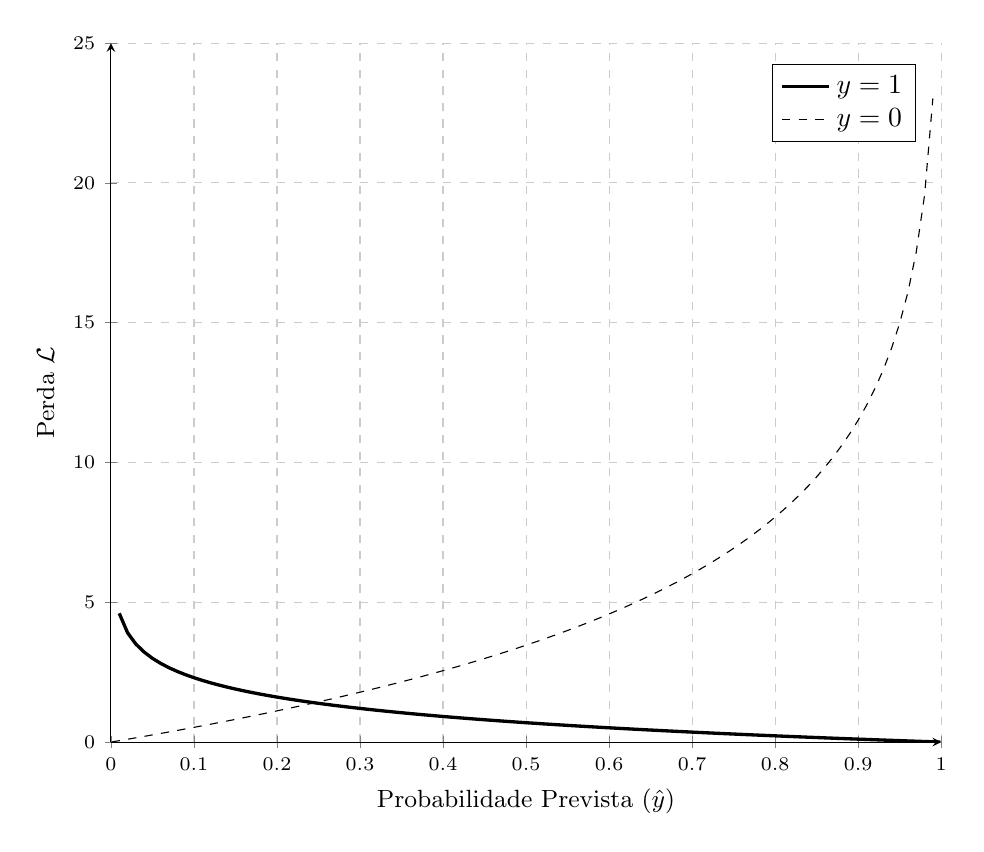
\begin{tikzpicture}
            \def\alphaZero{5.0} % Peso alto para a classe 0
            \def\alphaUm{1.0}   % Peso normal para a classe 1
            \begin{axis}[
                xlabel={Probabilidade Prevista ($\hat{y}$)},
                ylabel={Perda $\mathcal{L}$},
                axis lines=left,
                grid=major,
                grid style={dashed, gray!40},
                xmin=0, xmax=1,
                ymin=0, ymax=25, % Ajustar ymax para a curva mais íngreme
                legend pos=north east,
                width=\textwidth,
                label style={font=\small},
                tick label style={font=\scriptsize},
                title style={font=\bfseries, yshift=-5pt},
            ]
                % Curva para y=1
                \addplot[
                    domain=0.01:0.999, samples=100, color=black, very thick
                ] {-\alphaUm*ln(x)};
                \addlegendentry{$y=1$}

                % Curva para y=0
                \addplot[
                    domain=0.001:0.99, samples=100, color=black, dashed
                ] {-\alphaZero*ln(1-x)};
                \addlegendentry{$y=0$}
            \end{axis}
        \end{tikzpicture}
        \caption{Alto peso para a classe 0 ($\alpha_0=5.0, \alpha_1=1.0$).}
        \label{fig:comparativo-entropia-cruzada-ponderada-binaria-com-alto-peso-para-classe-0}
    \end{subfigure}
    \hfill 
    \begin{subfigure}[b]{0.48\textwidth}
        \centering
        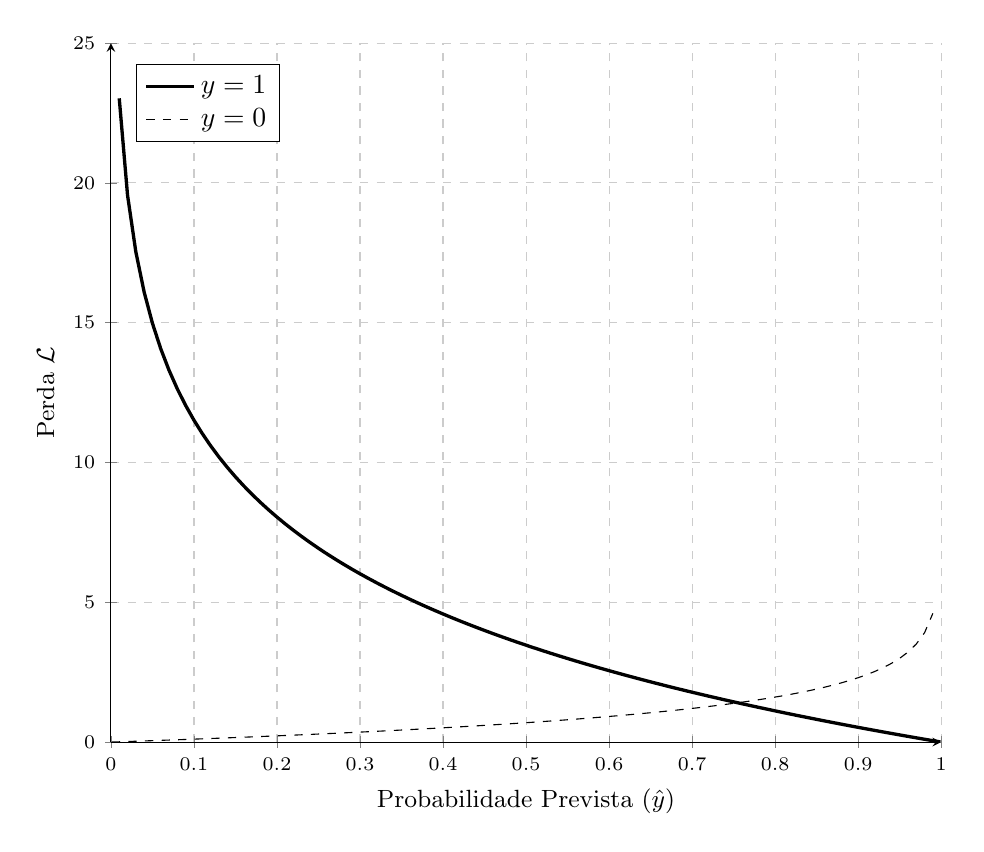
\begin{tikzpicture}
            \def\alphaZero{1.0} % Peso normal para a classe 0
            \def\alphaUm{5.0}   % Peso alto para a classe 1
            \begin{axis}[
                xlabel={Probabilidade Prevista ($\hat{y}$)},
                ylabel={Perda $\mathcal{L}$},
                axis lines=left,
                grid=major,
                grid style={dashed, gray!40},
                xmin=0, xmax=1,
                ymin=0, ymax=25, % Manter a mesma escala de y
                legend pos=north west,
                width=\textwidth,
                label style={font=\small},
                tick label style={font=\scriptsize},
                title style={font=\bfseries, yshift=-5pt},
            ]
                % Curva para y=1
                \addplot[
                    domain=0.01:0.999, samples=100, color=black, very thick
                ] {-\alphaUm*ln(x)};
                \addlegendentry{$y=1$}

                % Curva para y=0
                \addplot[
                    domain=0.001:0.99, samples=100, color=black, dashed
                ] {-\alphaZero*ln(1-x)};
                \addlegendentry{$y=0$}
            \end{axis}
        \end{tikzpicture}
        \caption{Alto peso para a classe 1 ($\alpha_0=1.0, \alpha_1=5.0$).}
        \label{fig:comparativo-entropia-cruzada-ponderada-binaria-com-alto-peso-para-classe-1}
    \end{subfigure}
    
    \caption{Visualizações da função de perda entropia-cruzada binária ponderada para diferentes valores de $\alpha_0$ e $\alpha_1$ }
    \label{fig:comparativo-entropia-cruzada-ponderada-binaria}
\end{figure}
\subsubsection*{Características da entropia-cruzada binária ponderada}

Por ser uma variante da BCE, a entropia-cruzada binária ponderada herda suas características da função primária. 

\begin{description}[style=sameline, leftmargin=1.5em, font=\bfseries\color{black}] 
    \item[Continuidade, suavidade e diferenciabilidade:] A WBCE é uma função de classe $C^{\infty}$, \textbf{infinitamente diferenciável} no domínio aberto $\hat{y}_i \in (0, 1)$ (ver Apêndice~\ref{ap:deducoes-perdas-derivadas-da-kl-divergence}). Dessa forma, ao utilizar a WBCE tanto com otimizadores baseados em gradiente, quanto em otimizadores de segunda ordem, não serão encontrados problemas de não-diferenciabilidade, facilitando a aplicação desses métodos.
    \item[Convexidade:] A WBCE é uma função \textbf{convexa} em relação predições $\hat{y}$ (ver Apêndice~\ref{ap:deducoes-perdas-derivadas-da-kl-divergence}). Esta é uma vantagem para a WBCE caso seja combinada com otimizadores baseados em gradiente. Contudo, devido às transformações não-lineares, sua convexidade pode ser afetada caso seja utilizada em redes neurais.
    \item[Robustez:] A WBCE não é Lipschitz-contínua, sendo \textbf{sensível a erros confiantes} (ver Apêndice~\ref{ap:deducoes-perdas-derivadas-da-kl-divergence}). Assim como BCE, erros confiantes do modelo podem enviesar o treinamento, gerando explosões de gradientes e o mal ajuste dos parâmetros da rede. Como a WBCE tem pesos, a classe em minoria irá apresentar um gradiente de crescimento mais acelerado, o que pode ser um problema caso os dados estejam rotulados incorretamente, aumentando o valor da perda.
\end{description}

\subsubsection*{Gradiente da entropia-cruzada binária ponderada}

A derivada parcial da WBCE em relação à predição é calculada através da Equação~\ref{eq:binary-weighted-cross-entropy-derivada}. Sua fórmula é semelhante à da BCE com a adição dos hiperparâmetros $\alpha$ que são tratados como constantes na diferenciação da Equação~\ref{eq:binary-weighted-cross-entropy}.

\begin{equacaodestaque}{Gradiente da entropia-cruzada binária ponderada em relação à predição}
    \nabla_{\hat{y}} \mathcal{L}_{\text{WBCE}} = \frac{\alpha_0(1-y)\hat{y} - \alpha_1 y(1-\hat{y})}{\hat{y}(1-\hat{y})}
    \label{eq:binary-weighted-cross-entropy-derivada}
\end{equacaodestaque}

De forma semelhante à BCE, a WBCE pode ser aplicada em conjunto com a sigmoide logística garantir a saída do modelo no intervalo $[0,1]$ e com isso, evitar o problema dos gradientes explosivos. Essa variante da derivada está na Equação~\ref{eq:wbce-gradiente-com-simgoide}.

\begin{equacaodestaque}{Gradiente da entropia-cruzada binária ponderada em relação à predição com sigmoide}
    \frac{\partial}{\partial \hat{y}} \mathcal{L}_{\text{wbce}} = 
        \begin{cases}
            \alpha_0 \cdot \hat{y} & \text{se} \quad y = 0 \\
            \alpha_1 \cdot (\hat{y} - 1) & \text{se} \quad y = 1 \\
        \end{cases}
    \label{eq:wbce-gradiente-com-simgoide}
\end{equacaodestaque}

Como a Figura~\ref{fig:binary-weighted-cross-entropy-derivada-comparacao} apresenta, as curvas do gradiente da WBCE também são assimétricas. A curva mais alta, é que possui o maior valor de $\alpha$. Ao gerar um gradiente em maior magnitude para a classe em minoria, a WBCE permite uma variação maior na atualização dos parâmetros para esse classe. A classe em maioria aparece mais, e consequentemente gera mais atualizações nos pesos e vieses. Ao adicionar pesos, a WBCE garante que as duas classes recebam o mesmo grau de importância. Essa ideia é parecida com a dos otimizadores baseados em gradientes adaptativos, como o AdaGrad, vistos no Capítulo~\ref{cap:retropropagacao-gradiente}. Nesse sentido, um gradiente maior, representa um ``passo'' maior, e uma curva mais íngreme, forçando o otimizador a fazer ajustes maiores para aprender os detalhes da classe em desvatagem.

\begin{figure}[h!]
    \centering
    \begin{subfigure}[b]{0.48\textwidth}
        \centering
        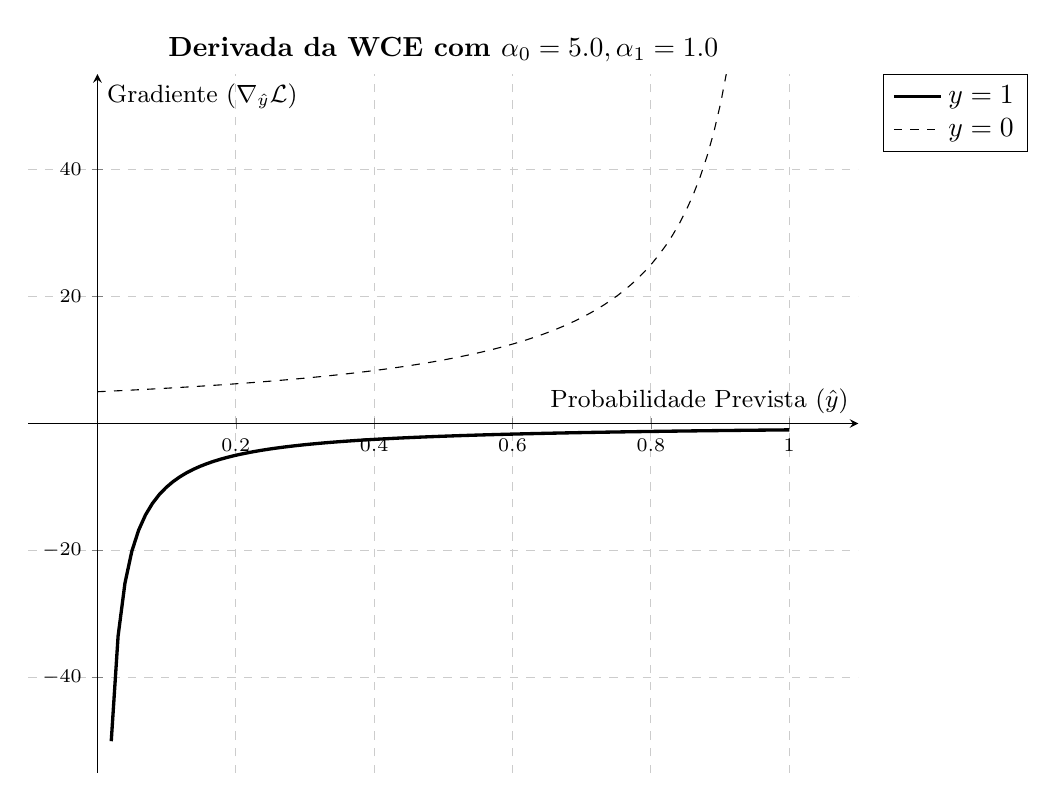
\begin{tikzpicture}
            \def\alphaZero{5.0} % Peso alto para a classe 0
            \def\alphaUm{1.0}   % Peso normal para a classe 1
            \begin{axis}[
                title={Derivada da WCE com $\alpha_0=5.0, \alpha_1=1.0$},
                xlabel={Probabilidade Prevista ($\hat{y}$)},
                ylabel={Gradiente ($\nabla_{\hat{y}} \mathcal{L}$)},
                axis lines=middle,
                grid=major,
                grid style={dashed, gray!40},
                xmin=-0.1, xmax=1.1,
                ymin=-55, ymax=55, % Aumentar range para ver o efeito
                legend pos=outer north east,
                width=\textwidth,
                label style={font=\small},
                tick label style={font=\scriptsize},
                title style={font=\bfseries, yshift=-5pt},
            ]
                % Derivada para y=1
                \addplot[
                    domain=0.02:1, samples=100, color=black, very thick
                ] {-\alphaUm/x};
                \addlegendentry{$y=1$}

                % Derivada para y=0
                \addplot[
                    domain=0:0.98, samples=100, color=black, dashed
                ] {\alphaZero/(1-x)};
                \addlegendentry{$y=0$}
            \end{axis}
        \end{tikzpicture}
        \caption{Gradiente amplificado para erros na classe 0.}
        \label{fig:wce-derivada-alpha0}
    \end{subfigure}
    \hfill
    \begin{subfigure}[b]{0.48\textwidth}
        \centering
        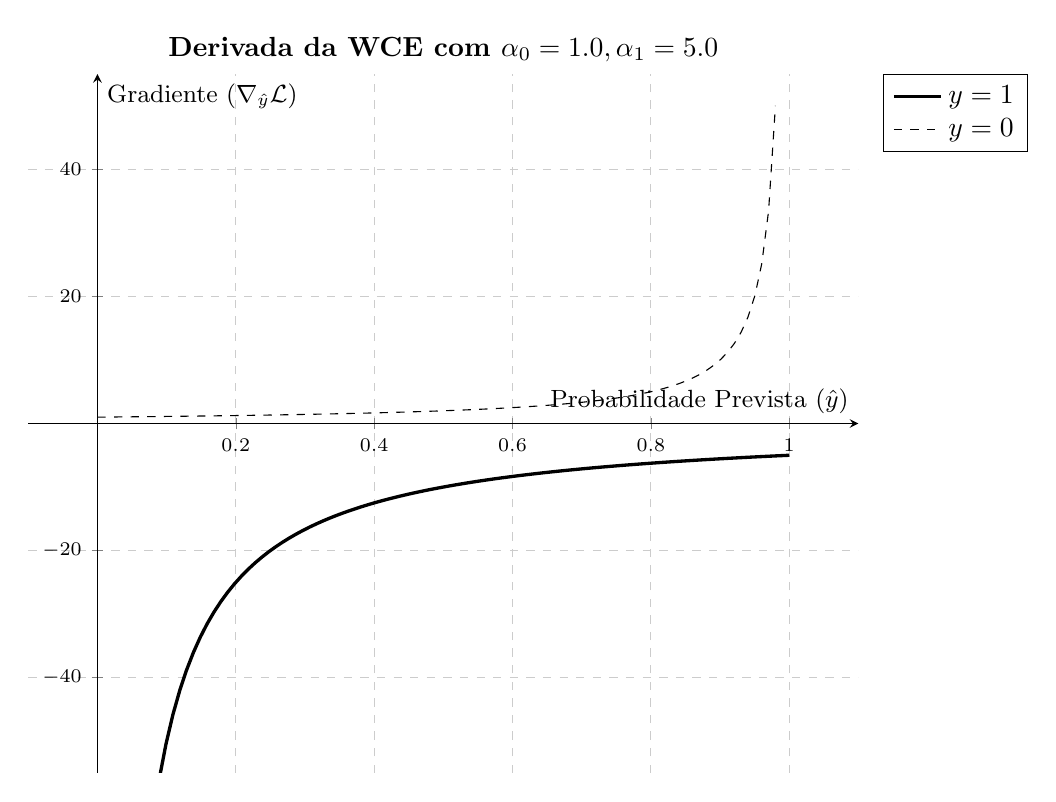
\begin{tikzpicture}
            \def\alphaZero{1.0} % Peso normal para a classe 0
            \def\alphaUm{5.0}   % Peso alto para a classe 1
            \begin{axis}[
                title={Derivada da WCE com $\alpha_0=1.0, \alpha_1=5.0$},
                xlabel={Probabilidade Prevista ($\hat{y}$)},
                ylabel={Gradiente ($\nabla_{\hat{y}} \mathcal{L}$)},
                axis lines=middle,
                grid=major,
                grid style={dashed, gray!40},
                xmin=-0.1, xmax=1.1,
                ymin=-55, ymax=55, % Manter a mesma escala de y
                legend pos=outer north east,
                width=\textwidth,
                label style={font=\small},
                tick label style={font=\scriptsize},
                title style={font=\bfseries, yshift=-5pt},
            ]
                % Derivada para y=1
                \addplot[
                    domain=0.02:1, samples=100, color=black, very thick
                ] {-\alphaUm/x};
                \addlegendentry{$y=1$}

                % Derivada para y=0
                \addplot[
                    domain=0:0.98, samples=100, color=black, dashed
                ] {\alphaZero/(1-x)};
                \addlegendentry{$y=0$}
            \end{axis}
        \end{tikzpicture}
        \caption{Gradiente amplificado para erros na classe 1.}
        \label{fig:wce-derivada-alpha1}
    \end{subfigure}
    
    \caption{Comparação do gradiente da entropia-cruzada ponderada para diferentes valores de $\alpha_0$ e $\alpha_1$.}
    \label{fig:binary-weighted-cross-entropy-derivada-comparacao}
\end{figure}

\subsubsection*{Aplicações da entropia-cruzada binária ponderada}%
\index{Aplicações práticas! Entropia-cruzada binária ponderada}

\begin{description}[style=sameline, leftmargin=1.5em, font=\bfseries\color{black}] 
    \item[Identificação de doenças toráxicas em raios-x (Saúde):] \textcite{li2025chex} criam um modelo de \textit{ensamble} em uma \textit{DenseNet} para identificar doenças em raios-x de tórax, como o \textit{dataset} utilizado, o NIH ChestX-ray14, apresenta dados que seguem uma distribuição assimétrica de cauda longa, os autores combinam a WBCE com a perda assimétrica para lidar com desequilíbrio de classes.
    \item[Segmentação de lesões de degeneração macular (Saúde):] \textcite{starodub2025surpassingstateartamd} criam arquiteturas U-Net para a segmentação de lesões de degeneração macular relacionada à idade (AMD), os autores optam pela WBCE ao invés da \textit{dice loss} pelo fato da segunda tender a ser instável em primeiros planos esparsos (\textit{sparse foregrounds}) devido à sua sensibilidade a erros de predição pequenos.
    \item[Detecção de mudanças em imagens de satélite (Sensoriamento remoto)] \textcite{naveed2025adaptingsamcrossentropymasking} comparam a performance da WBCE com uma função de perda chamada \textit{Cross-Entropy Masking} (CEM) no Levir-CD \textit{dataset}, um conjunto de dados para treinar modelos de sensoriamento remoto, com objetivo de detectar pequenas mudanças nas imagens.
\end{description}

\subsection{Perda hinge (Hinge loss)}%
\index{Funções de Perda!Perda hinge}

A \textbf{perda \textit{hinge}} é função de perda para de máquinas de vetores de suporte para classificação binária, sendo proposta no artigo \textit{Support-Vector Networks} dos autores \textcite{HingeLoss}. No trabalho, \textcite{HingeLoss} analisam um conjunto de dados que não pode ser separado sem erros, de forma que os autores querem separá-los gerando a menor quantidade possível de erros. Para isso, \textcite{HingeLoss} introduzem um conjunto de variáveis não-negativas $\xi_i \ge 0, i = 1, 2, \cdots, l$, e também a função que querem minimizar, denotada por

\[
    `\Phi ' = \sum_{i = 1}^l \xi_i^{\sigma}
\]

Para $\sigma > 0$, são sujeitas as restrições

\[
    y_i (\textbf{w} \cdot \textbf{x}_i + b) \ge 1 - \xi_i, i = 1, 2, \cdots, l
\]

\[
    \xi \ge 0, i = 1, 2, \cdots, l
\]

Para que $\xi$ siga as restrições propostas, ele deve ser maior ou igual às restrições. Como ele deve ser o menor possível para minimizar o erro, seu menor tamanho é o máximo entre 0 e $1 - y(\textbf{w} \cdot \textbf{x}_i + b)$. Escrevemos algo da forma

\[
    \xi = \max (0, 1 - y(\textbf{w} \cdot \textbf{x}_i + b))
\]

Essa função encontrada ao buscar o mínimo entre esses dois termos, ficou conhecida como \textbf{\textit{hinge loss}}. A Equação~\ref{eq:hinge-loss} descreve essa função com as notações desta obra.

\begin{equacaodestaque}{Perda hinge}
    \mathcal{L}_{\text{hinge}} (y, f(x)) = \max(0, 1 - y \cdot f(x))
    \label{eq:hinge-loss}
\end{equacaodestaque}

Em que

\begin{description}[style=sameline, leftmargin=1.5em, font=\bfseries\color{black}] 
    \item[$y$] representa os rótulos dos dados, segue o formato $y \in {-1, +1}$;
    \item[$f(x)$] representa a saída bruta do modelo ou a função de decisão (geralmente the signed distance da barreira de decisão)
\end{description}

A perda \textit{hinge} tem três comportamentos distintos com base nas predições do modelo:

\begin{enumerate}
    \item \textbf{Correta e confiante ($y \cdot f(x) \ge 1$)}: gera uma perda nula. Se o ponto classificado foi classificado com a classe correta e está longe da fronteira nada deve ser feito.
    \item \textbf{Correta, mas arriscada ($0 < y \cdot f(x) < 1$)}: gera uma perda positiva. O ponto foi classificado com a classe correta, mas está dentro da margem. O modelo é forçado a empurrar a margem para mais longe desses pontos.
    \item \textbf{Incorreta ($y \cdot f(x) \ge 0$)}: Gera uma perda que cresce linearmente com base no erro do modelo.
\end{enumerate}

Dessa forma, ao ser utilizada em uma SVM, a perda \textit{hinge} atua com o objetivo de maximizar a margem e fazer com que o modelo encontre o melhor hiperpalano que separe corretamente as duas classes de dados. Quando a \textit{hinge} penaliza predições corretas mas pouco confiantes, ela cria um corredor mais largo entre as classes. Isso melhora a generalizações do modelo, dado que ele não fica ajustado apenas aos dados de treino, mas é criada uma margem segura para novos dados.

Uma analogia para explicar o conceito por trás da perda \textit{hinge} é pensarmos em uma estrada de mão dupla. A perda \textit{hinge} não quer que estejamos apenas do lado correto, ela maximiza a margem, garantindo um espaço seguro do carro à linha do centro da pista. Mesmo dirigindo do lado correto, se estiver próximo do centro da pista, você será penalizado, esse seria o cenário da predição correta porém arriscada. Dessa forma, a \textit{hinge} atua consideravelmente diferente das perdas probabilísticas, como a BCE, ao calcular a distância entre duas distribuições de Bernoulli.

Diferente dos gráficos da BCE que apresentam curvas suaves devido ao uso dos logaritmos, a Figura~\ref{fig:hinge-loss} evidencia que a perda \textit{hinge} é composta por retas. Mais precisamente, essa função de perda tem o formato de uma dobradiça, por isso recebe o nome \textit{hinge}. Assim como a perda $\epsilon$-insensível, que apresenta uma ``zona morta'', a \textit{hinge} também tem essa característica, a perda cresce linearmente, mas quando as predições estão corretas, é garantido uma zona de perda zero.

\begin{figure}
    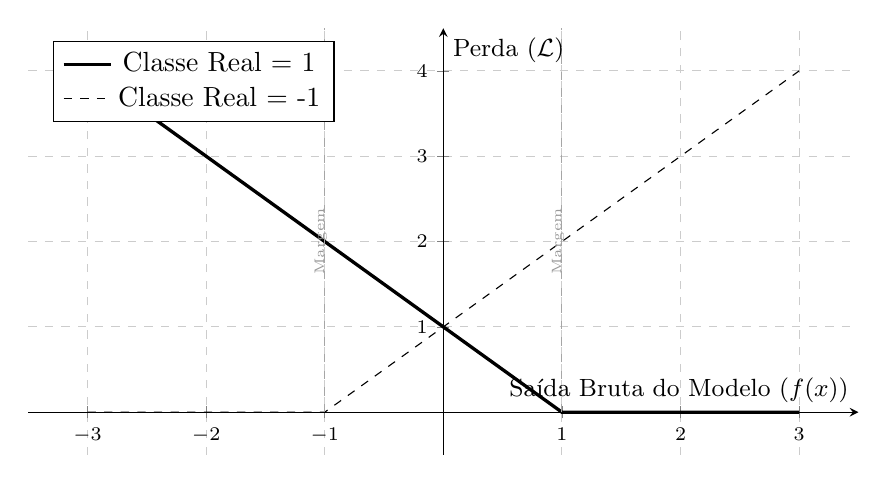
\begin{tikzpicture}
    \begin{axis}[
        xlabel={Saída Bruta do Modelo ($f(x)$)},
        ylabel={Perda ($\mathcal{L}$)},
        axis lines=middle,
        grid=major,
        grid style={dashed, gray!40},
        xmin=-3.5, xmax=3.5,
        ymin=-0.5, ymax=4.5,
        legend pos=north west,
        width=\linewidth,
        height=7cm,
        title style={font=\bfseries},
        label style={font=\small},
        tick label style={font=\scriptsize}
        ]
        % Curva para a classe real y=+1
        \addplot[
            domain=-3:3,
            samples=100,
            color=black,
            very thick
            ] {max(0, 1-x)};
        \addlegendentry{Classe Real = 1}

        % Curva para a classe real y=-1
        \addplot[
            domain=-3:3,
            samples=100,
            color=black,
            dashed
            ] {max(0, 1+x)};
        \addlegendentry{Classe Real = -1}

        % Opcional: Linhas tracejadas para marcar as margens
        \draw[dashed, gray!70] (axis cs:1, 0) -- (axis cs:1, 4.5);
        \draw[dashed, gray!70] (axis cs:-1, 0) -- (axis cs:-1, 4.5);
        \node[above, gray!80, font=\tiny, rotate=90] at (axis cs:1.1, 2) {Margem};
        \node[above, gray!80, font=\tiny, rotate=90] at (axis cs:-0.9, 2) {Margem};
    \end{axis}
    \end{tikzpicture}
    \caption{Visualização da função de perda \textit{hinge} no plano.}
    \label{fig:hinge-loss}
    \fonte{O autor (2025).}
\end{figure}

\subsubsection*{Características da perda hinge}

\begin{description}[style=sameline, leftmargin=1.5em, font=\bfseries\color{black}] 
    \item[Continuidade, suavidade e diferenciabilidade:] A perda \textit{hinge} é uma função de classe $C^0$, \textbf{contínua} (ver Apêndice~\ref{ap:deducoes-perda-hinge}). Por utilizar a função $\max$ em sua fórmula, essa função de perda apresenta uma ``quinas'' em seu relevo, fazendo com que a perda \textit{hinge} não seja totalmente suave. Um fato que pode dificultar a otimização utilizando métodos de segunda ordem.
    \item[Convexidade:] A perda \textit{hinge} é uma função \textbf{convexa} (ver Apêndice~\ref{ap:deducoes-perda-hinge}). A função $\max$ une duas funções convexas, garantindo como resultado uma função também convexa. Ao utilizar a perda \textit{hinge} em máquinas de vetores de suporte, é possível garantir um único ponto de mínimo.
    \item[Robustez:] A perda Hinge é uma função 1-Lipschitz-contínua, portanto, é \textbf{robusta a erros confiantes} (ver Apêndice~\ref{ap:deducoes-perda-hinge}). Ao derivar a perda \textit{hinge} e calcular o seu gradiente no infinito, é visto que ele não cresce indefinidamente. Pelo contrário, ele fica constante em 1.
    \item[Esparsidade:] Semelhante a perda $\epsilon$-insensível (ver Seção-xx) a perda \textit{hinge} promove gradientes esparsos (ver Apêndice~\ref{ap:deducoes-perda-hinge}). Isso se dá devido à uma zona de perda zero que ocorre com o objetivo de separar os vetores de suporte. Neste caso, os vetores de suporte são os que estão dentro da margem ou foram classificados incorretamente. Ao definir quais são os vetores de suporte, a perda \textit{hinge} faz uma distinção entre os classificações fáceis (perda zero), das predições difíceis. Assim, os vetores de suporte deixam claro para o modelo quais classificações devem ser melhoradas, diferente de perdas como a BCE, que geram gradientes pequenos para todos os pontos, até mesmo os fáceis. Isso mantém o modelo ``ocupado'' em tentar melhorar todas as predições, a esparsidade da \textit{hinge} evita esse fenômeno.
\end{description}

\subsubsection*{Gradiente da perda hinge}

Da perda \textit{hinge} calculamos o seu gradiente em relação à saída bruta do modelo $f(x)$, o qual é dado através de uma função por partes. Como essa função apresenta um ponto de não-diferenciabilidade no caso $y \cdot f(x) = 1$ utilizamos o subgradiente para definir o intervalo de resultados possíveis para a derivada neste ponto. Essa derivada está na Equação~\ref{eq:hinge-loss-derivada}

\begin{equacaodestaque}{Gradiente da perda hinge em relação à saída bruta do modelo}
    \nabla_{f(x)} \mathcal{L} = 
    \begin{cases} 
      -y & \text{se } y \cdot f(x) < 1 \\
      0 & \text{se } y \cdot f(x) > 1 \\
      [-y, 0] & \text{se } y \cdot f(x) = 1
    \end{cases}
    \label{eq:hinge-loss-derivada}
\end{equacaodestaque}

Mesmo a definição correta para a derivada da perda \textit{hinge} no caso que $y \cdot f(x) = 1$ seja qualquer resultado no intervalo [-y, 0], bibliotecas como PyTorch e TensorFlow implementam essa decisão de forma arbitrária, considerando o gradiente como sendo 0 ou $y$. Uma situação semelhante acontece ao derivar a função de ativação ReLU.

Além da Equação~\ref{eq:hinge-loss-derivada} que já evidencia a continuidade de Lipschitz, a Figura~\ref{fig:hinge-loss-derivada-grafico} trás essa propriedade de forma gráfica. Na derivada, a perda \textit{hinge} deixa de ser duas retas conectas e torna-se uma espécie de degrau unitário para o cálculo do gradiente.

\begin{figure}[h!]
    \centering
    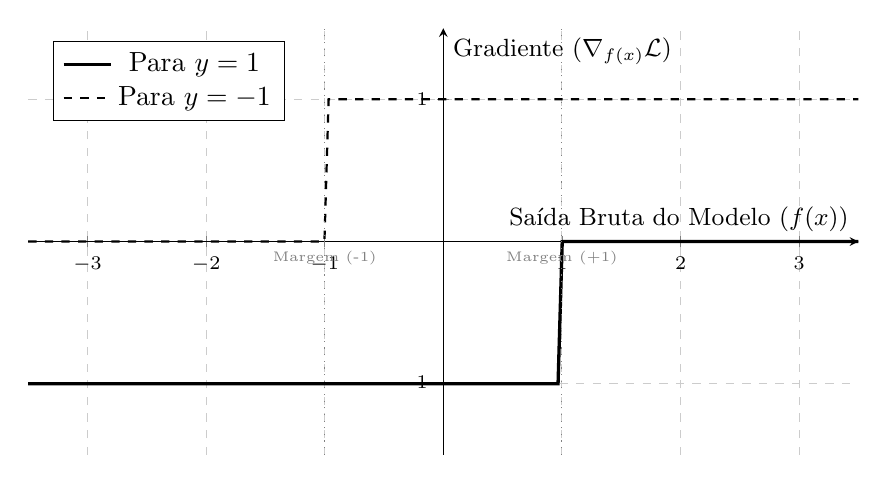
\begin{tikzpicture}
        \begin{axis}[
            width=\linewidth,
            height=7cm,
            xlabel={Saída Bruta do Modelo ($f(x)$)},
            ylabel={Gradiente ($\nabla_{f(x)} \mathcal{L}$)},
            axis lines=middle,
            grid=major,
            grid style={dashed, gray!40},
            xmin=-3.5, xmax=3.5,
            ymin=-1.5, ymax=1.5, % Ajustado para mostrar valores negativos e positivos
            ytick={-1, 0, 1}, % Mostra apenas os valores relevantes no eixo Y
            legend pos=north west,
            title style={font=\bfseries},
            label style={font=\small},
            tick label style={font=\scriptsize}
        ]
        % --- CASO 1: Classe Real y = +1 ---
        % Se f(x) < 1, gradiente é -1. Se f(x) > 1, gradiente é 0.
        \addplot[
            domain=-3.5:3.5,
            samples=200,
            color=black,
            very thick
            ] {
            (x < 1) * -1 + (x >= 1) * 0
            };
        \addlegendentry{Para $y = 1$}

        % --- CASO 2: Classe Real y = -1 ---
        % Se f(x) > -1, o erro cresce com x, logo gradiente é +1.
        % Se f(x) < -1, o erro é 0, logo gradiente é 0.
        \addplot[
            domain=-3.5:3.5,
            samples=200,
            color=black,
            dashed,
            thick
            ] {
            (x > -1) * 1 + (x <= -1) * 0
            };
        \addlegendentry{Para $y = -1$}

        % Linhas verticais de guia para as margens (opcional, ajuda a leitura)
        \draw[dotted, gray] (axis cs:1, -1.5) -- (axis cs:1, 1.5);
        \draw[dotted, gray] (axis cs:-1, -1.5) -- (axis cs:-1, 1.5);
        % Labels pequenos para indicar onde a margem "quebra"
        \node[below, gray, font=\tiny] at (axis cs:1, 0) {Margem (+1)};
        \node[below, gray, font=\tiny] at (axis cs:-1, 0) {Margem (-1)};

        \end{axis}
    \end{tikzpicture}
    \caption{Relação linear por partes do gradiente da função de perda \textit{hinge}.}
    \label{fig:hinge-loss-derivada-grafico}
    \fonte{O autor (2025).}
\end{figure}

\subsubsection*{Aplicações da perda hinge}%
\index{Aplicações práticas! Perda hinge}

A perda \textit{hinge} foi amplamente utilizada na criação das máquinas de vetores de suporte. Contudo, sua não-diferenciabilidade afeta negativamente que técnicas de otimização, como o gradiente descendente, sejam aplicadas com sucesso. Assim, surgem diversas variantes da perda \textit{hinge} que buscam estender seus conceitos de maximização de margem e ao mesmo tempo garantir uma função suave e diferenciável.

\begin{description}[style=sameline, leftmargin=1.5em, font=\bfseries\color{black}] 
    \item[Variante huberizada da perda \textit{hinge} (Aprendizado de máquina):] \textcite{Xu_2015} aborda as dificuldades de se utilizar a perda \textit{hinge} nas SVMs devido à sua não-diferenciabilidade em partes da função, o autor utiliza uma versão huberizada da perda \textit{hinge}, semelhante a perda de Huber (ver Seção-xx) que atua de forma quadrática para erros pequenos e linear para erros grandes. A versão huberizada da perda \textit{hinge} permite o uso do método do gradiente proximal (PG) com um tempo de convergência linear \parencite{Xu_2015}.
    \item[Variante suave da perda \textit{hinge} em classificação de textos (Aprendizado de máquina):] \textcite{luo2021learningsmoothhingelosses} apresentam duas perdas \textit{hinge} suaves que são infinitamente diferenciáveis obtendo duas máquinas de vetores de suporte suaves (SSVMs), os autores testam as SSVMs em tarefas de classificação de texto concluindo que os algoritmos criados são efetivos para aplicações do mundo real.
    \item[Variante sensível a custos da perda \textit{hinge} (Aprendizado de máquina):] \textcite{masnadishirazi2015costsensitivesupportvectormachines} estendem os conceitos da perda \textit{hinge} criando uma variante sensível ao custo (\textit{cost sensitive}), os autores explicam que cenários como diagnósticos médicos, detecção de fraudes e tomada de decisão de negócios uma falha, como um falso positivo pode afetar drasticamente mais que um falso positivo. Nessas situações a \textit{cost sensitive hinge loss} consegue minimizar o custo e o risco melhor que a perda \textit{hinge} tradicional \parencite{masnadishirazi2015costsensitivesupportvectormachines}. 
\end{description}

\subsection{Perda hinge quadrática (Squared hinge loss)}

A perda \textit{hinge} foi amplamente utilizada na construção das SVMs. Contudo, como visto nas aplicações dessa função, o seu ponto de não-diferenciabilidade em $y - \cdot f(x) = \pm 1$ afeta a otimização através do gradiente. Assim, com o passar do tempo foram surgindo alternativas para a perda \textit{hinge} que corrigem seus problemas de suavidade. Ainda em \textit{Support-Vector Networks}, mesmo artigo em que \textcite{HingeLoss} propõem a \textit{hinge}, os autores citam uma outra função da forma

\[
    \frac{1}{2} \textbf{w}^2 + CF \left( \sum_{i = 1}^l \xi_i^{\sigma} \right)
\]

no qual $F(u)$ é uma função convexa monotônica e $C$ é uma constante.

Quando $\sigma = 1$ temos o cálculo da perda \textit{hinge} vista anteriormente. Contudo, quando $\sigma = 2$ temos a \textit{hinge} quadrática. No artigo, os autores focam em trabalhar com a perda \textit{hinge} para evitar lidar com um problema NP-Completo \parencite{HingeLoss}. Mesmo sendo não sendo trabalhada em maior profundidade no artigo de Vapnik, não demorou muito para que outros autores experimentassem outros índices para $\sigma$. Foi isso que aconteceu em \textit{Lagrangian support vector machines}, no trabalho \textcite{mangasarian2001lagrangian} utilizam a \textbf{perda \textit{hinge} quadrática}, levando-os para um algoritmo de interação lagraniano para otimização da perda. Ao mudar a função de perda, o problema passa a envolver uma matriz positiva definida, permitindo que a otimização seja feita de forma simples e rápida resolvendo um sistema de equações lineares \parencite{mangasarian2001lagrangian}.

A perda \textit{hinge} quadrática trouxe para as máquinas de vetores de suporte um novo paradigma de otimização devido à sua suavidade. Essa função é definida como o quadrado da perda \textit{hinge}, como visto na Equação~\ref{eq:squared-hinge-loss}.

\begin{equacaodestaque}{Perda hinge quadrática}
    \mathcal{L}_{\text{hinge}^2}(y, f(x)) = (\max(0, 1 - y \cdot f(x)))^2
    \label{eq:squared-hinge-loss}
\end{equacaodestaque}

Por utilizar um termo quadrático para avaliar a perda, a Figura~\ref{fig:squared-hinge-loss} mostra que a perda \textit{hinge} quadrática possui um comportamento de curvas suaves. Desse modo, ela resolve o problema da não-diferenciabilidade no ponto $1 - y \cdot f(x) = 1$, permitindo que métodos de primeira ordem não encontrem problemas ao otimizar a função. Por outro lado, o erro cresce de forma mais acelerada que na perda \textit{hinge} tradicional, apresentando consequências no quesito de robustez da \textit{hinge} quadrática.

\begin{figure}[h!]
    \centering
    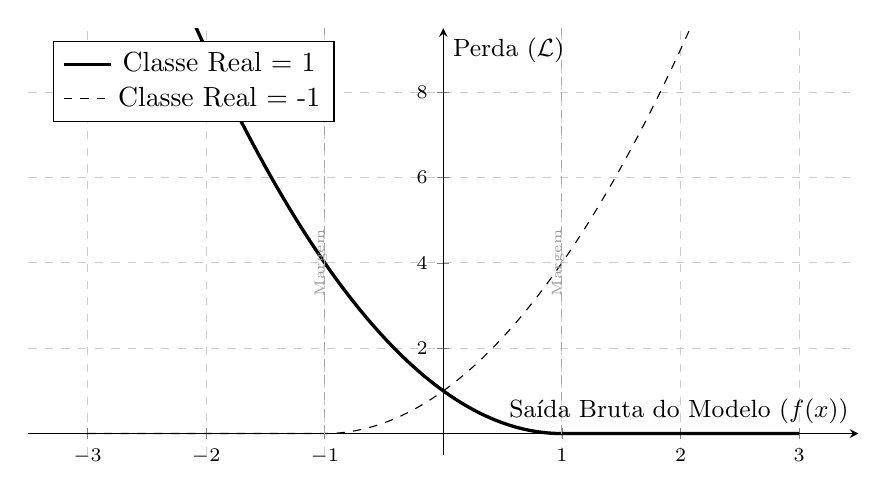
\begin{tikzpicture}
        \begin{axis}[
            xlabel={Saída Bruta do Modelo ($f(x)$)},
            ylabel={Perda ($\mathcal{L}$)},
            axis lines=middle,
            grid=major,
            grid style={dashed, gray!40},
            xmin=-3.5, xmax=3.5,
            ymin=-0.5, ymax=9.5,       
            legend pos=north west,
            width=\linewidth,
            height=7cm,
            title style={font=\bfseries},
            label style={font=\small},
            tick label style={font=\scriptsize}
        ]
            % Curva para a classe real y=+1
            \addplot[
                domain=-3:3, 
                samples=201, % Aumentei os samples para uma curva mais suave
                color=black, 
                very thick
            ] {(max(0, 1-x))^2}; % Adicionado o ^2
            \addlegendentry{Classe Real = 1}

            % Curva para a classe real y=-1
            \addplot[
                domain=-3:3, 
                samples=201, 
                color=black, 
                dashed
            ] {(max(0, 1+x))^2}; % Adicionado o ^2
            \addlegendentry{Classe Real = -1 }
            
            % Linhas tracejadas para marcar as margens
            \draw[dashed, gray!70] (axis cs:1, 0) -- (axis cs:1, 9.5);
            \draw[dashed, gray!70] (axis cs:-1, 0) -- (axis cs:-1, 9.5);
            \node[above, gray!80, font=\tiny, rotate=90] at (axis cs:1.1, 4) {Margem};
            \node[above, gray!80, font=\tiny, rotate=90] at (axis cs:-0.9, 4) {Margem};
            
        \end{axis}
    \end{tikzpicture}
    \caption{Visualização da função perda hinge quadrática no plano.}
    \label{fig:squared-hinge-loss}
    \fonte{O autor (2025).}
\end{figure}

\subsubsection*{Características da perda hinge quadrática}

\begin{description}[style=sameline, leftmargin=1.5em, font=\bfseries\color{black}] 
    \item[Continuidade, suavidade e diferenciabilidade:] A perda \textit{hinge} quadrática é uma função de classe $C^1$, \textbf{suave} (ver Apêndice~\ref{ap:deducoes-perda-hinge-quadratica}). Ao elevar a perda \textit{hinge} ao quadrado, é garantido uma função suave e sem ``bicos'', como resultado, não é necessário o uso de subgradiente para calcular as derivadas parciais da perda. Assim, métodos mais simples de otimização podem ser aplicados com essa perda.
    \item[Convexidade:] A perda \textit{hinge} quadrática é uma função \textbf{convexa} (ver Apêndice~\ref{ap:deducoes-perda-hinge-quadratica}). Desse modo, essa função de perda garante apenas um ponto de mínimo global, facilitando a otimização dos parâmetros do modelo.
    \item[Robustez:] A perda \textit{hinge} quadrática não é Lipschitz-contínua, sendo \textbf{sensível a erros confiantes} (ver Apêndice~\ref{ap:deducoes-perda-hinge-quadratica}). Quando a perda \textit{hinge} quadrática é derivada, os termos quadráticos tornam-se retas que tendem ao infinito conforme as probabilidades do modelo aumentam. Assim, erros confiantes podem enviesar o cálculo do gradiente, e até causar problemas de gradientes explosivos.
\end{description}

\subsubsection*{Gradiente da perda hinge quadrática}

O cálculo das derivadas perda \textit{hinge} quadrática são mais simples que a função original. Para encontrar a derivada parcial em relação à saída do modelo devemos aplicar a regra da cadeia, separando o termo quadrático da perda \textit{hinge}. Fazendo isso, encontramos a Equação~\ref{eq:squared-hinge-loss-derivada}. No caso da perda \textit{hinge} tradicional, é visto que ela consegue escrever a derivada com apenas duas condições, não sendo necessária uma condição específica para $y \cdot f(x) = 1$. Isso justifica a não utilização do subgradiente na derivação.

\begin{equacaodestaque}{Gradiente da perda hinge quadrática}
    \nabla_{f(x)} \mathcal{L}_{\text{hinge}^2} = 
    \begin{cases} 
        -2y(1 - y \cdot f(x)) & \text{se } y \cdot f(x) < 1 \\
        0 & \text{se } y \cdot f(x) \ge 1
    \end{cases}
    \label{eq:squared-hinge-loss-derivada}
\end{equacaodestaque}

A Figura~\ref{fig:squared-hinge-loss-derivada} mostra que o gradiente da perda \textit{hinge} quadrática cresce indefinidamente conforme os valores da saída do modelo aumentam, isso evidencia o fato dessa função de perda não ser Lipschitz-contínua como a perda \textit{hinge} tradicional.

\begin{figure}[h!]
    \centering
    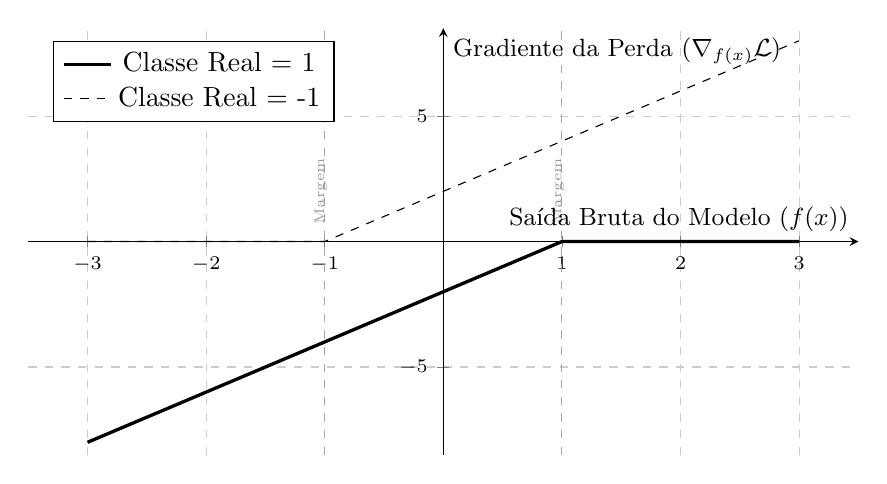
\begin{tikzpicture}
        \begin{axis}[
            xlabel={Saída Bruta do Modelo ($f(x)$)},
            ylabel={Gradiente da Perda ($\nabla_{f(x)} \mathcal{L}$)},
            axis lines=middle,
            grid=major,
            grid style={dashed, gray!40},
            xmin=-3.5, xmax=3.5,
            ymin=-8.5, ymax=8.5,         % Ajustar o y para a escala linear da derivada
            legend pos=north west,
            width=\linewidth,
            height=7cm,
            title style={font=\bfseries},
            label style={font=\small},
            tick label style={font=\scriptsize}
        ]
            % Derivada para a classe real y=+1
            % Fórmula: (x < 1) ? (2*(x-1)) : 0
            \addplot[
                domain=-3:3, 
                samples=10, 
                color=black, 
                very thick
            ] {(x < 1) ? (2*(x-1)) : 0};
            \addlegendentry{Classe Real = 1}

            % Derivada para a classe real y=-1
            % Fórmula: (x > -1) ? (2*(x+1)) : 0
            \addplot[
                domain=-3:3, 
                samples=10, 
                color=black, 
                dashed
            ] {(x > -1) ? (2*(x+1)) : 0};
            \addlegendentry{Classe Real = -1}
            
            % Linhas tracejadas para marcar as margens
            \draw[dashed, gray!70] (axis cs:1, -8.5) -- (axis cs:1, 8.5);
            \draw[dashed, gray!70] (axis cs:-1, -8.5) -- (axis cs:-1, 8.5);
            \node[above, gray!80, font=\tiny, rotate=90] at (axis cs:1.1, 2) {Margem};
            \node[above, gray!80, font=\tiny, rotate=90] at (axis cs:-0.9, 2) {Margem};
            
        \end{axis}
    \end{tikzpicture}
    \caption{Representação gráfica da derivada da função de perda Squared Hinge Loss. O gradiente é proporcional à distância da margem.}
    \label{fig:squared-hinge-loss-derivada}
    \fonte{O autor (2025).}
\end{figure}

\subsubsection*{Aplicações da perda hinge quadrática}%
\index{Aplicações práticas! Perda hinge quadrática}

\begin{description}[style=sameline, leftmargin=1.5em, font=\bfseries\color{black}] 
    \item[SVMs com perda \textit{hinge} norma-$p$ (Área):] \textcite{sun2024psvmsoftmarginsvmspnorm} discutem as $p$SVMs, as quais generalizam a margem suave das SVMs ao introduzir a perda \textit{hinge} norma-$p$, essa nova função de perda tem um parâmetro $p$ cujo objetivo é elevar a perda \textit{hinge} ao exponente $p$. Os autores explicam que ao utilizar a perda \textit{hinge} norma-$p$ com $p = 1$ (perda \textit{hinge}) ou $p = 2$ (perda \textit{hinge} quadrática) o algoritmo de otimização SMO é simplificado em uma expressão linear, garantindo uma performance mais eficiente \parencite{sun2024psvmsoftmarginsvmspnorm}.
    \item[\textit{Gradient boosting} com perda \textit{hinge} quadrática (Área):] \textcite{zeng2020fullycorrectivegradientboostingsquared} propõem um algoritmo de \textit{boosting} para classificação binária que utiliza a perda \textit{hinge} quadrática, como justificativa, os autores explicam que essa função permite o princípio da margem.
    \item[Comparativo de funções de perda para classifação em aprendizado profundo (Área):] \textcite{janocha2017lossfunctionsdeepneural} investigam como a escolha de funções de perda afetam modelos profundos e suas dinâmicas de aprendizado, em testes realizados pelos autores foi concluído que a perda \textit{hinge} quadrática gerou modelos que poderiam ser treinados mais rapidamente quando comparada com outras funções, como a entropia-cruzada e a perda $L_1$. Além disso, as perdas que trabalham com a maximização da margem possuem a tendência de generalizar melhor, ultrapassando as outras famílias analisadas \parencite{janocha2017lossfunctionsdeepneural}.
\end{description}

\section{Funções de perda para classificação multi-classe}

As perdas vistas até o momento são utilizadas em cenários nos quais temos apenas duas classes para serem identificadas. Mas, vão existir situações onde teremos um conjunto maior de classes para serem analisadas. Nesses casos, utilizaremos perdas de classificação multi-classe, como a entropia-cruzada categóricas e as suas variações. 

\subsection{Exemplo ilustrativo:}

\subsection{Entropia-cruzada categórica (CCE)}%
\index{Funções de Perda!Entropia-cruzada categórica (CCE)}

A entropia-cruzada categórica, também chamada de \textbf{\textit{categorical cross-entropy}} (\textbf{CCE}), estende os conceitos da BCE para lidar com $C$ diferentes classes em uma representação em formato \textit{one-hot}. A formatação \textit{one-hot} funciona da seguinte forma: para cada uma das classes presentes, é adicionada uma coluna binária responsável por marcar 1 se há presença daquela classe, ou 0, se há ausência da classe. Um exemplo dessa codificação está na Tabela~\ref{tab:one-hot-encoding-exemplo}.

\begin{table}[htbp]
    \centering
    \begin{threeparttable}
        \caption{Exemplo da codificação \textit{one-hot}.}%
        \label{tab:one-hot-encoding-exemplo}
        \begin{tabular}{l c c c c }
            \toprule
            Cor original & cor\_vermelho & cor\_azul & cor\_verde \\
            \midrule
            Vermelho & 1 & 0 \\
            Azul & 0 & 1 & 0 \\
            Verde & 0 & 0 & 1 \\
            \bottomrule
        \end{tabular}
        
        \begin{tablenotes}[para]
            \small
            \item[] Fonte: O autor (2025).
        \end{tablenotes}

    \end{threeparttable}
\end{table}

A Equação~\ref{eq:categorical-cross-entropy} representa o cálculo da CCE para $C$ classes. Diferente da BCE que era escrita com o cálculo de duas entropias-cruzadas, a CCE deixa esse cálculo implícito com o uso da notação de somatória. Mas, para cada uma das classes existentes no problema analisado, existirá uma entropia-cruzada, que somadas, chegarão na perda por uma amostra.

\begin{equacaodestaque}{Entropia-cruzada categórica}
    \mathcal{L}_{cce} (y, \hat{y}) = - \sum_{c=1}^{C} y_c \log(\hat{y}_c)
    \label{eq:categorical-cross-entropy}
\end{equacaodestaque}

Em que

\begin{description}[style=sameline, leftmargin=1.5em, font=\bfseries\color{black}] 
    \item[$y_j$] representa o valor real da j-ésima amostra;
    \item[$\hat{y}_j$] representa o valor predito pelo modelo;
    \item[$N$] representa o número de amostras.
\end{description}

Representar o gráfico da CCE em uma figura é algo complexo, visto que, ele pode variar conforme o número de classes existentes. Considerando isso, a Figura~\ref{fig:categorical-cross-entropy} apresenta o gráfico contendo apenas uma entropia-cruzada, com a sua curva logarítmica. Note que o gráfico é o mesmo da entropia-cruzada binária, visto que a CCE é uma estensão dessa outra função de perda.

\begin{figure}

    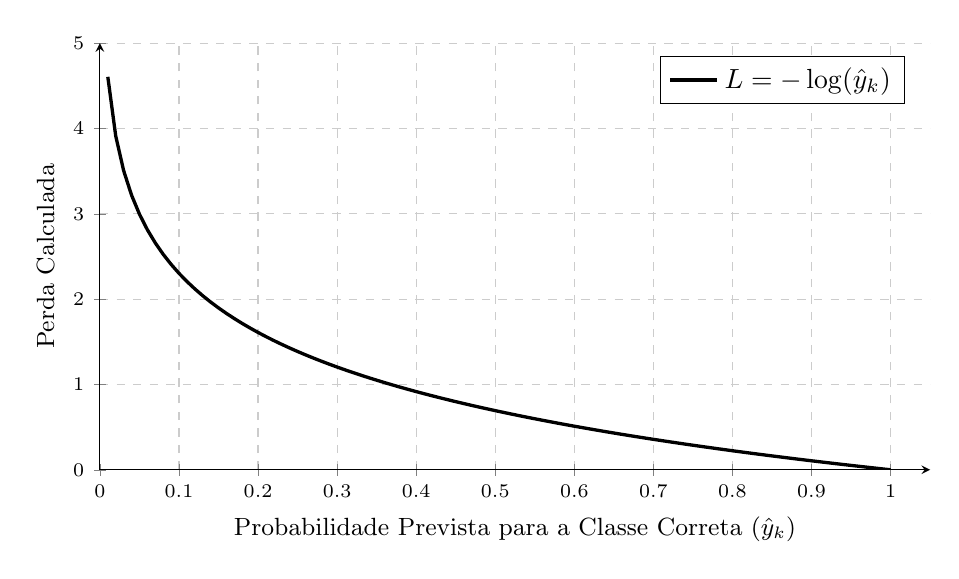
\begin{tikzpicture}
        \begin{axis}[
            xlabel={Probabilidade Prevista para a Classe Correta ($\hat{y}_k$)},
            ylabel={Perda Calculada},
            axis lines=left,              % Eixos no canto inferior esquerdo
            grid=major,                   % Adiciona uma grade principal
            grid style={dashed, gray!40},   % Estilo da grade
            xmin=0, xmax=1.05,            % Limites do eixo x
            ymin=0, ymax=5,               % Limites do eixo y
            legend pos=north east,        % Posição da legenda
            width=\linewidth,
            height=7cm,           
            title style={font=\bfseries},
            label style={font=\small},
            tick label style={font=\scriptsize}
        ]
            % Plota a função -log(y_k_hat)
            \addplot[
                domain=0.01:1, % Domínio para evitar log(0)
                samples=100,
                color=black,
                very thick
            ] {-ln(x)};
            
            \addlegendentry{$L = -\log(\hat{y}_k)$}
            
        \end{axis}
    \end{tikzpicture}

    \caption{Visualização da função de perda entropia-cruzada categórica no plano.}
    \label{fig:categorical-cross-entropy}
    \fonte{O autor (2025).}

\end{figure}

\subsubsection*{Características da entropia-cruzada categórica}

A CCE herda da entropia-cruzada binária diversas propriedades matemáticas, como a lista explicita.

\begin{description}[style=sameline, leftmargin=1.5em, font=\bfseries\color{black}] 
    \item[Continuidade, suavidade e diferenciabilidade:] A CCE é de classe $C^{\infty}$, \textbf{infinitamente diferenciável} no domínio aberto $\hat{y}_i \in (0, 1)$ (ver Apêndice~\ref{ap:deducoes-perdas-derivadas-da-kl-divergence}). Por ser infinitamente diferenciável, não são encontradas dificuldades ao calcular as derivadas da CCE, seja as derivadas de primeira ordem, para métodos baseados em gradiente. Quanto derivadas de segunda ordem, para o método de Newton e relacionados.
    \item[Convexidade:] A CCE é \textbf{convexa} em relação predições $\hat{y}$ (ver Apêndice~\ref{ap:deducoes-perdas-derivadas-da-kl-divergence}). Ao ser classificada como convexa, a CCE garante apenas um ponto de mínimo global, facilitando a otimização utilizando gradiente. Contudo, a convexidade pode ser alterada caso seja utilizada em aprendizado profundo.
    \item[Robustez:] A CCE não é Lipschitz-contínua, sendo \textbf{sensível a erros confiantes} (ver Apêndice~\ref{ap:deducoes-perdas-derivadas-da-kl-divergence}). Essa também é uma característica que a CCE herda da BCE, algo que pode enviesar o cálculo do gradiente e até causar problemas de gradientes explosivos.
    \item[Saída softmax:] Semelhante a BCE, a qual aceitava valores entre 0 e 1 e por isso precisava de ser utilizada junto com a sigmoide logística, a entropia cruzada categórica também tem requisitos parecidos. Como um modelo de rede neural geralmente retorna como saída \textit{logits} $z_i \in \mathbb{R}^C$, ao utilizar uma função \textit{softmax} é possível garantir que a $\sum_{j} \hat{p}_{i,j} = 1$, ou seja, que xxxx \parencite{LossesArticle}.
    \item[Penalização alta para erros confiantes:] Como \textcite{LossesArticle} explicam, a entropia cruzada categórica segue a mesma ideia da entropia cruzada binária, de forma que essa função também tem como propriedade punir os erros confiantes de forma mais elevada.
    \item[Requisitos \textit{one-hot}] Como dito anteriormente a CCE aceita um vetor em formato \textit{one-hot}, isso significa que os valores tanto para $y_j$ quanto para $\hat{y}_j$ devem estar em formato de probabilidade, estando em valores entre zero e um \footnote{Para trabalhar com valores em que os rótulos estão organizados com valores inteiros é possível utilizar uma variante da \textit{categorical cross-entropy}: a \textit{sparse cross-entropy}. Essa função está melhor explicada na Seção \ref{sec:sparse-cross-entropy}}.
\end{description}

\subsubsection*{Gradiente da entropia-cruzada categórica}

A derivada parcial da CCE em relação a predição $\hat{y}_c$ está representada na Equação~\ref{eq:derivada-cce-direta}.

\begin{equation}
    \frac{\partial \mathcal{L}_{cce}}{\partial \hat{y}_c} = - \frac{y_c}{\hat{y}_c}
    \label{eq:derivada-cce-direta}
\end{equation}

Contudo, também consideraremos o cenário em que essa função de perda é aplicada em conjunto com a função de ativação \textit{softmax} na saída do modelo. Primeiro, relembramos a equação da \textit{softmax} dada por

\[
    \mathcal{A}_{\text{softmax}}(z_i) = \frac{e^{z_i}}{\sum_{j=1}^{K} e^{z_j}}
\]

Primeiro, aplicamos a regra da cadeia, pois, a CCE depende das previsões $\hat{y}_j$ e as previsões, por sua vez, dependem dos \textit{logits}. Escrevemos a regra da cadeia como sendo

\[
    \frac{\partial \mathcal{L}}{\partial z_i} = \sum_{j=1}^{C} \frac{\partial \mathcal{L}}{\partial \hat{y}_j} \cdot \frac{\partial \hat{y}_j}{\partial z_i}
\]

Calculamos a derivada em relação à previsão, ou seja, $\partial \mathcal{L} / \partial \hat{y}_j$, assim, escrevemos

\[
    \frac{\partial \mathcal{L}}{\partial \hat{y}_j} = \frac{\partial}{\partial \hat{y}_j} \left( - \sum_{k=1}^{C} y_k \log(\hat{y}_k) \right) = -y_j \cdot \frac{1}{\hat{y}_j} = -\frac{y_j}{\hat{y}_j}
\]

Calculamos também a a derivada da função \textit{softmax} considerando dois diferentes casos, quando $i = j$, ou seja derivada da saída de uma classe em relação à sua própria entrada de \textit{logit}, assim, utilizando a regra do quociente chegamos na expressão

\[
    \frac{\partial \hat{y}_i}{\partial z_i} = \frac{e^{z_i}(\sum_k e^{z_k}) - e^{z_i} \cdot e^{z_i}}{(\sum_k e^{z_k})^2}
\]

Simplificando a expressão uma primeira vez temos

\[
    \frac{e^{z_i}}{\sum_k e^{z_k}} - \left( \frac{e^{z_i}}{\sum_k e^{z_k}} \right)^2
\]

Chegamos então nos termos

\[
    \hat{y}_i - \hat{y}_i^2 = \hat{y}_i (1 - \hat{y}_i)
\]

Já para o caso em que que é calculada a derivada da saída de uma classe em relação à entrada de \textit{logit} de outra classe, ou seja $i \neq j$ a equação é dada por

\[
    \frac{\partial \hat{y}_j}{\partial z_i} = \frac{0 \cdot (\sum_k e^{z_k}) - e^{z_j} \cdot e^{z_i}}{(\sum_k e^{z_k})}
\]

Simplificando ela, encontramos em

\[
    - \left( \frac{e^{z_j}}{\sum_k e^{z_k}} \right) \left( \frac{e^{z_i}}{\sum_k e^{e_z}} \right) = -\hat{y}_j \hat{y}_i
\].

O próximo passo é substituir as derivadas parciais calculadas na regra da cadeia, para isso será separado o somatório nos casos em que $i = j$ e nos casos que $i \neq = j$.

\[
    \frac{\partial \mathcal{L}}{\partial z_i} = \left( \frac{\partial \mathcal{L}}{\partial \hat{y}_i} \cdot \frac{\partial \hat{y}_i}{\partial z_i} \right) + \sum_{j \neq i} \left( \frac{\partial \mathcal{L}}{\partial \hat{y}_j} \cdot \frac{\partial \hat{y}_j}{\partial z_i} \right)
\]

Substituindo os resultados encontrados temos

\[
    \left( - \frac{y_i}{\hat{y}_i} \cdot \hat{y}_i (1 - \hat{y}_i) \right) + \sum_{j \neq i} \left( - \frac{y_j}{\hat{y}_j} \cdot (-\hat{y}_j\hat{y}_i) \right)
\]

Simplificamos os termos escrevendo

\[
    - y_i (1 - \hat{y}_i) + \sum_{j \neq i} (y_j \hat{y}_i)
\]

Aplicamos a distributiva encontrando

\[
    - y_i + y_i \hat{y}_i + \hat{y}_i \sum_{j \neq i} y_j
 \]

$y$ representa um vetor \textit{one-hot encoded}, o qual contém todas as probabilidades para cada uma das classes que o modelo está analisando, isso significa que a soma de todos esses elementos vai ser 1. Com isso, escrevemos que $\sum_{j = 1}^C y_j = 1$. Contudo, na expressão que está sendo desenvolvida nós temos todos os elementos exceto pelo o i-ésimo, portanto: $\sum_{j\neq i} y_j = 1 - y_i$.

Substituindo essa informação na equação temos

 \[
    y_i + y_i \hat{y}_i + \hat{y}_i (1 - y_i)
 \]

 Aplicando mais uma vez a distributiva para expandir o termo $\hat{y}_i (1 - y_i)$:

 \[
    -y_i + y_i \hat{y}_i + \hat{y}_i - y_i \hat{y}_i
 \]

 Perceba que os termos $y_i \hat{y}_i $ e $y_i \hat{y}_i$ se cancelam, então é possível chegar na expressão \ref{eq:category-cross-entropy-derivada}. A qual representa a derivada da \textit{categorical cross-entropy} para um cenário em que o último componente do modelo é a função de ativação softmax. Note que ao invés de ser uma derivada complexa como nos outros casos vistos até agora, a derivada da CCE passa a ser apenas o cálculo da diferença entre os valores preditos e os valores reais.

\begin{equacaodestaque}{Gradiente entropia-cruzada categórica para a Softmax}
    \nabla_{z_i} \mathcal{L} (y, \hat{y}) = \hat{y}_i - y_i
    \label{eq:category-cross-entropy-derivada}
\end{equacaodestaque}

Note também que a que essa simplificação dos cálculos para a derivada na entropia cruzada utilizando a \textit{softmax} também reflete no gráfico, que é composto apenas de , como é possível ver na Figura \ref{fig:categorical-cross-entropy-derivada-com-softmax}.

\begin{figure}[h!]
    \centering
    \begin{tikzpicture}
        \begin{axis}[
            xlabel={Probabilidade Prevista para a Classe $i$ ($\hat{y}_i$)},
            ylabel={Gradiente da Perda ($\frac{\partial L}{\partial z_i}$)},
            axis lines=middle,             % Eixos centrados em (0,0)
            grid=major,                  % Adiciona uma grade principal
            grid style={dashed, gray!40},  % Estilo da grade
            xmin=-0.1, xmax=1.1,           % Limites do eixo x
            ymin=-1.1, ymax=1.1,           % Limites do eixo y
            legend pos=north west,         % Posição da legenda
            width=\linewidth,
            height=7cm,                   % Altura do gráfico
            title style={font=\bfseries},
            label style={font=\small},
            tick label style={font=\scriptsize}
        ]
            % Curva para a classe correta (y_i = 1)
            % A derivada é y_hat - 1
            \addplot[
                domain=0:1,
                samples=10,
                color=black,
                very thick
            ] {x - 1};
            \addlegendentry{Classe Correta ($y_i=1 \implies \hat{y}_i - 1$)}

            % Curva para uma classe incorreta (y_i = 0)
            % A derivada é y_hat - 0
            \addplot[
                domain=0:1,
                samples=10,
                color=black,
                dashed
            ] {x};
            \addlegendentry{Classe Incorreta ($y_i=0 \implies \hat{y}_i - 0$)}
            
        \end{axis}
    \end{tikzpicture}
    \caption{Representação gráfica da derivada da \textit{categorical cross entropy} com Softmax.}
    \label{fig:categorical-cross-entropy-derivada-com-softmax}
    \fonte{O autor (2025).}
\end{figure}

Caso a \textit{categorical cross entropy} não seja utilizada em conjunto com a função de ativação \textit{softmax} na saída do modelo, a sua derivada passa a ser um pouco mais complexa, sendo representada pela Equação \ref{eq:categorical-cross-entropy-derivada}.

\begin{equacaodestaque}{Gradiente da entropia-cruzada categórica em relação à predição}
    \nabla_{\hat{y}_i} \mathcal{L}_{\text{cce}} = -\frac{y_i}{\hat{y}_i}
    \label{eq:categorical-cross-entropy-derivada}
\end{equacaodestaque}

\subsubsection*{Aplicações da entropia-cruzada categórica}%
\index{Aplicações práticas! Entropia Cruzada Categórica}

\begin{description}[style=sameline, leftmargin=1.5em, font=\bfseries\color{black}] 
    \item[Aplicação 1 (Área):]
    \item[Aplicação 2 (Área):]
    \item[Aplicação 3 (Área):]
\end{description}

Conhecida a CCE, uma das principais funções de perda para ser utilizada para problemas de classificação multi-classe, é possível se perguntar: O que acontece se os dados não estiverem codificados em formato \textit{one-hot}? Para contornar esse problema, uma solução é utilizar a \textit{sparse categorical cross-entropy}, a qual será explicada em sequência.

\subsection{Entropia-cruzada categórica esparsa (Sparse CCE)}%
\index{Funções de Perda!Entropia-cruzada categórica esparsa (Sparse CCE)}%
\label{sec:sparse-cross-entropy}

A entropia cruzada categórica esparsa é utilizada para os cenários em que os rótulos das classes são dados em inteiros $y_j \in {1, 2, \cdots C}$ \parencite{LossesArticle}. A \textit{sparse CCE} para um conjunto de individual de predição é dada pela Equação \ref{eq:sparse-categorical-cross-entropy-per-sample}

\begin{equacaodestaque}{Entropia-cruzada categórica esparsa para uma amostra $j$}
    \mathcal{L}_{\text{sparse cce}}(y, \hat{y}) = - \sum_{c=1}^{C} y_c \log(\hat{y}_c)
    \label{eq:sparse-categorical-cross-entropy-per-sample}
\end{equacaodestaque}

Perceba que as fórmulas da \textit{sparse categorical cross entropy} são iguais as da sua versão para rótulos codificados para formato \textit{one-hot}, por isso os seus gráficos também serão iguais, assim, o próximo passo é discutir algumas das características dessa função de perda.

\subsubsection*{Características da entropia-cruzada categórica esparsa}

\begin{description}[style=sameline, leftmargin=1.5em, font=\bfseries\color{black}] 
    \item[Continuidade, suavidade e diferenciabilidade:] A CCE esparsa é de classe $C^{\infty}$, \textbf{infinitamente diferenciável} no domínio aberto $\hat{y}_i \in (0, 1)$ (ver Apêndice~\ref{ap:deducoes-perdas-derivadas-da-kl-divergence}).
    \item[Convexidade:] A CCE esparsa é \textbf{convexa} em relação predições $\hat{y}$ (ver Apêndice~\ref{ap:deducoes-perdas-derivadas-da-kl-divergence}).
    \item[Robustez:] A CCE esparsa não é Lipschitz-contínua, sendo \textbf{sensível a erros confiantes} (ver Apêndice~\ref{ap:deducoes-perdas-derivadas-da-kl-divergence}).
    \item[Eficiência:] \textcite{LossesArticle} explicam que em problemas de classificação com um grande número de classes, a codificação \textit{one-hot} pode ser memória-intensiva, ao utilizar a \textit{sparse CCE}, os seus indexes que já apontam diretamente para a probabilidade conseguem escapar de trabalhar com dados em formato \textit{one-hot}.
    \item[Similaridades com a CCE:]  A \textit{sparse CCE} possui grandes similaridades com a CCE original, isso significa que vantagens como a diferenciabilidade e a penalização de erros muito confiantes que são características da \textit{categorical cross entropy}, também estão presentes na sua versão esparsa.
\end{description}

Além dessa variante, a \textit{categorical cross-entropy} possui uma versão que faz uso de pesos para as classes, buscando trabalhar com casos em que existe uma presença maior de algumas classes do que de outras. Essa é a \textit{weighted categorical cross-entropy}, que será vista em seguida.

\subsubsection*{Aplicações da Entropia-Cruzada Categórica Esparsa}%
\index{Aplicações práticas! Entropia Cruzada Categórica Esparsa}

\begin{description}[style=sameline, leftmargin=1.5em, font=\bfseries\color{black}] 
    \item[Aplicação 1 (Área):]
    \item[Aplicação 2 (Área):]
    \item[Aplicação 3 (Área):]
\end{description}

\subsection{Entropia-cruzada categórica ponderada (WCCE)}%
\index{Funções de Perda!Entropia-cruzada categórica ponderada (WCCE)}

A fórmula da \textit{weighted categorical cross-entropy} lembra bastante a fórmula da \textit{weighted binary cross-entropy}, pois sua única diferença com a variante original é a adição de um peso multiplicando o erro para aquela classe. Essa função de perda para uma amostra $j$ é dada pela Equação \ref{eq:weighted-categorical-cross-entropy-per-sample}.

\begin{equacaodestaque}{Entropia-cruzada categórica Ponderada}
    \mathcal{L}_{\text{wcce}}(y, \hat{y}) = - \sum_{c=1}^{C} \alpha y_c \log(\hat{y}_c)
    \label{eq:weighted-categorical-cross-entropy-per-sample}
\end{equacaodestaque}

Em que

\begin{description}[style=sameline, leftmargin=1.5em, font=\bfseries\color{black}] 
    \item[$y_j$] representa o valor real da j-ésima amostra;
    \item[$\hat{y}_j$] representa o valor predito pelo modelo;
    \item[$N$] representa o número de amostras.
\end{description}

\subsubsection*{Características da entropia-cruzada categórica ponderada}

\begin{description}[style=sameline, leftmargin=1.5em, font=\bfseries\color{black}] 
    \item[Continuidade, suavidade e diferenciabilidade:] A WCCE é de classe $C^{\infty}$, \textbf{infinitamente diferenciável} no domínio aberto $\hat{y}_i \in (0, 1)$ (ver Apêndice~\ref{ap:deducoes-perdas-derivadas-da-kl-divergence}).
    \item[Convexidade:] A WCCE é \textbf{convexa} em relação predições $\hat{y}$ (ver Apêndice~\ref{ap:deducoes-perdas-derivadas-da-kl-divergence}).
    \item[Robustez:] A WCCE não é Lipschitz-contínua, sendo \textbf{sensível a erros confiantes} (ver Apêndice~\ref{ap:deducoes-perdas-derivadas-da-kl-divergence}).
\end{description}

Assim, de forma semelhante à \textit{weighted binary cross-entropy} é possível utilizar a sua variante multi-classe para ser trabalhada em cenários em que uma classe, ou um grupo de classes aparece de forma mais frequente que outro.

\subsubsection*{Aplicações da Entropia-Cruzada Categórica Ponderada}%
\index{Aplicações práticas! Entropia Cruzada Categórica Ponderada}

\begin{description}[style=sameline, leftmargin=1.5em, font=\bfseries\color{black}] 
    \item[Aplicação 1 (Área):]
    \item[Aplicação 2 (Área):]
    \item[Aplicação 3 (Área):]
\end{description}

\section{Perda multi-rótulo (multilabel loss)}%
\index{Funções de Perda!Multilabel Loss}

\begin{equacaodestaque}{Perda multi-rótulo}
    \mathcal{L}_{\text{multilabel}} = - \sum_{j=1}^{q} [y_j \log(\hat{y}_j) + (1 - y_j) \log(1 - \hat{y}_j)]
    \label{eq:multilabel-loss}
\end{equacaodestaque}

\begin{figure}[h!]
    \centering
    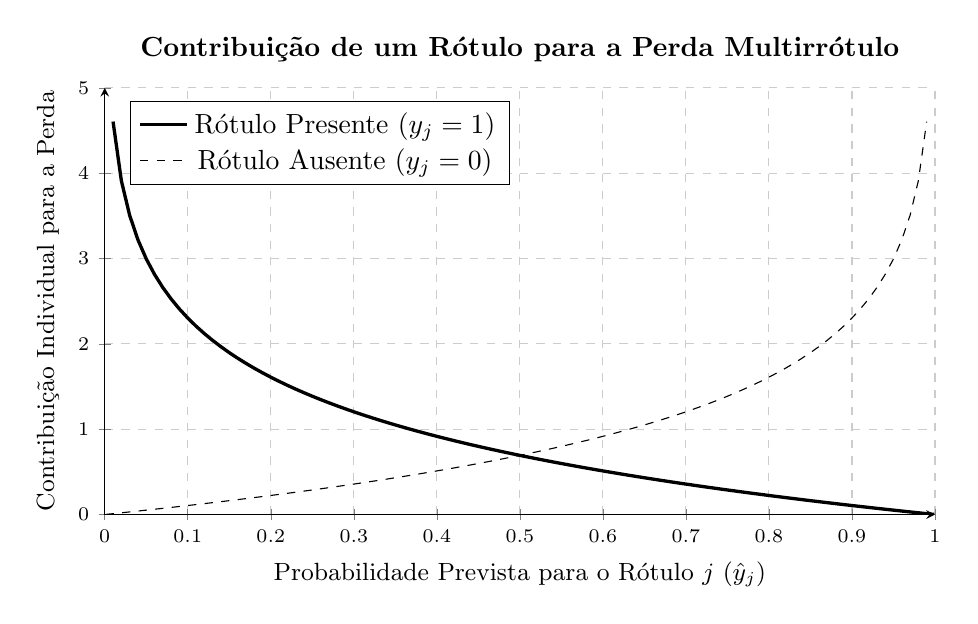
\begin{tikzpicture}
        \begin{axis}[
            title={Contribuição de um Rótulo para a Perda Multirrótulo},
            xlabel={Probabilidade Prevista para o Rótulo $j$ ($\hat{y}_j$)},
            ylabel={Contribuição Individual para a Perda},
            axis lines=left,
            grid=major,
            grid style={dashed, gray!40},
            xmin=0, xmax=1,
            ymin=0, ymax=5,
            legend pos=north west,
            width=\linewidth,
            height=7cm,
            title style={font=\bfseries},
            label style={font=\small},
            tick label style={font=\scriptsize}
        ]
            % Curva para quando o rótulo está presente (y_j = 1)
            \addplot[
                domain=0.01:0.999, samples=100, color=black, very thick
            ] {-ln(x)};
            \addlegendentry{Rótulo Presente ($y_j=1$)}

            % Curva para quando o rótulo está ausente (y_j = 0)
            \addplot[
                domain=0.001:0.99, samples=100, color=black, dashed
            ] {-ln(1-x)};
            \addlegendentry{Rótulo Ausente ($y_j=0$)}
            
        \end{axis}
    \end{tikzpicture}
    \caption{A perda multi-rótulo é a soma das contribuições de cada rótulo individual, que se comportam como a BCE.}
    \label{fig:multilabel-loss}
    \fonte{O autor (2025).}
\end{figure}

\subsubsection*{Características da perda multi-rótulo}

\begin{description}[style=sameline, leftmargin=1.5em, font=\bfseries\color{black}] 
    \item[Continuidade, suavidade e diferenciabilidade:] A perda multi-rótulo uma função de classe $C^\infty$, \textbf{infinitamente diferenciável}, no hipercubo aberto $(0, 1)^q$ (ver Apêndice~\ref{ap:deducoes-multilabel-loss}).
    \item[Convexidade:] A perda multi-rótulo é uma função \textbf{convexa} em relação ao vetor de predições $\mathbf{\hat{y}}$ (ver Apêndice~\ref{ap:deducoes-multilabel-loss}).
    \item[Robustez:] A perda multi-rótulo não é Lipschitz-contínua (ver Apêndice~\ref{ap:deducoes-multilabel-loss}).
\end{description}

\subsubsection*{Gradiente da perda multi-rótulo}

\begin{equacaodestaque}{Derivada da Perda Multirrótulo}
    \nabla_{z_i} \mathcal{L}_{\text{Multilabel}}= \hat{y}_i - y_i
    \label{eq:multilabel-loss-derivada}
\end{equacaodestaque}

\begin{figure}[h!]
    \centering
    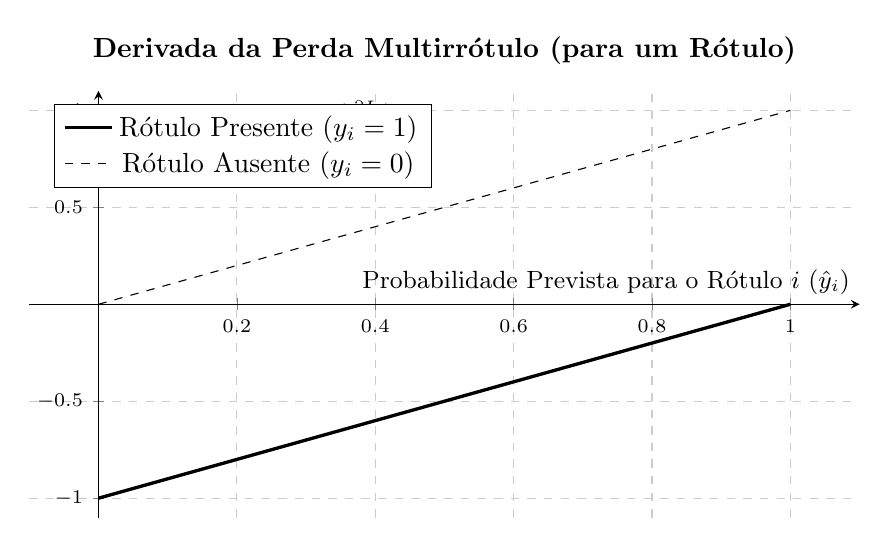
\begin{tikzpicture}
        \begin{axis}[
            title={Derivada da Perda Multirrótulo (para um Rótulo)},
            xlabel={Probabilidade Prevista para o Rótulo $i$ ($\hat{y}_i$)},
            ylabel={Gradiente da Perda ($\frac{\partial L}{\partial z_i}$)},
            axis lines=middle,
            grid=major,
            grid style={dashed, gray!40},
            xmin=-0.1, xmax=1.1,
            ymin=-1.1, ymax=1.1,
            legend pos=north west,
            width=\linewidth,
            height=7cm,
            title style={font=\bfseries},
            label style={font=\small},
            tick label style={font=\scriptsize}
        ]
            % Curva para rótulo presente (y_i = 1)
            \addplot[domain=0:1, samples=10, color=black, very thick] {x - 1};
            \addlegendentry{Rótulo Presente ($y_i=1$)}

            % Curva para rótulo ausente (y_i = 0)
            \addplot[domain=0:1, samples=10, color=black, dashed] {x};
            \addlegendentry{Rótulo Ausente ($y_i=0$)}
            
        \end{axis}
    \end{tikzpicture}
    \caption{O gradiente para cada rótulo é simplesmente a diferença entre a probabilidade prevista e o valor real (0 ou 1).}
    \label{fig:multilabel-loss-derivada}
    \fonte{O autor (2025).}
\end{figure}

\subsubsection*{Aplicações da perda multi-rótulo}%
\index{Aplicações práticas! Multi-label}

\begin{description}[style=sameline, leftmargin=1.5em, font=\bfseries\color{black}] 
    \item[Aplicação 1 (Área):]
    \item[Aplicação 2 (Área):]
    \item[Aplicação 3 (Área):]
\end{description}

\section{Comparativo: funções de perda para classificação}

\begin{table}[htbp]
    \centering
    \begin{threeparttable}
        \caption{Comparativo das funções de perda para problemas de classificação}
        \label{tab:comparativo-funcoes-de-perda-para-classificacao}
        % p{3.2cm} define uma largura fixa para a primeira coluna.
        % As 3 colunas 'X' restantes dividem o espaço que sobra de forma flexível.
        % >{\raggedright\arraybackslash} alinha o texto à esquerda para melhor leitura.
        \begin{tabularx}{\textwidth}{p{3.2cm} *{1}{>{\raggedright\arraybackslash}X}}
            \toprule
            \textbf{Função} & \textbf{Principais Características} \\
            \midrule
            Entropia Cruzada Binária (BCE) & - \\
            \addlinespace
            entropia cruzada binária ponderada (\textit{WBCE}) & - \\
            \addlinespace
            Perda Hinge (\textit{Hinge Loss}) & - \\
            \addlinespace
            Entropia Cruzada Categórica (CCE) & -  \\
            \addlinespace
            Entropia Cruzada categórica Esparsa (\textit{Sparse CCE}) & - \\
            \addlinespace
            Entropia Cruzada Categórica Ponderada (\textit{WCCE}) & - \\
            \addlinespace
            Perda Multirrótulo (\textit{Multilabel Loss}) & - \\
            \addlinespace
        \end{tabularx}
        
        \begin{tablenotes}[para]
            \small
            \item[] Fonte: O autor (2025).
        \end{tablenotes}

    \end{threeparttable}
\end{table}

\section{Fluxograma: Escolhendo a Função de Perda Ideal}
